\documentclass[12pt,a4paper,twoside]{book}
\usepackage{graphicx}
\usepackage[utf8]{inputenc}
\usepackage[british]{babel}
\usepackage[colorlinks=true, linkcolor=blue, citecolor=blue, urlcolor=blue]{hyperref}
\usepackage{indentfirst}
\usepackage{amssymb}
\usepackage{amsmath}
\usepackage{latexsym}
\usepackage{lipsum}
\usepackage{tikz}
\usepackage{amsthm}
\usepackage{algorithm}
\usepackage{algpseudocode}
\usepackage{stmaryrd}
\usepackage{listings}
\usepackage{xcolor, colortbl}
\usepackage{pgfgantt}
\usepackage{dirtree}
\usepackage{todonotes}
\usepackage{bussproofs}
\usepackage{mathtools}
\usepackage{msc}
\usepackage{subcaption}
\usepackage{macros}
\usepackage[a4paper,inner=3.5cm,outer=2.5cm]{geometry}
\usepackage[titletoc,title,toc,page]{appendix}
\usepackage{verbatim}
\usepackage{placeins}
\usepackage{parskip}
\usepackage{blindtext}
\usepackage{chngcntr}
\counterwithin{table}{chapter}
\usepackage{newlfont}
\usepackage{fancyhdr}
\usepackage{float}
\usepackage[capitalize,noabbrev]{cleveref}
\usepackage{soul}
\usepackage[font=footnotesize,labelfont=bf]{caption}
\usepackage{multirow}
\usepackage{pdfpages}
\usepackage{sansmath}
% \usepackage{hyphenat}
% \hyphenation{mate-mati-ca recu-perare}

\newcommand{\rom}[1]{\uppercase\expandafter{\romannumeral #1\relax}}

\newtheorem{theorem}{Theorem}
\newtheorem{lemma}{Lemma}
\newtheorem{corollary}{Corollary}
\theoremstyle{definition}
\newtheorem{example}{Example}[section]

\usetikzlibrary{automata,arrows,positioning,shapes,snakes}
\usetikzlibrary{calc,matrix,decorations.pathmorphing}
\usetikzlibrary{shapes.geometric,arrows.meta}
\pgfmathtruncatemacro\distance{1}

\definecolor{green}{rgb}{0,0.5,0}
\definecolor{red}{rgb}{1,0,0}
\definecolor{yellow}{rgb}{0.5,0.5,0}
\definecolor{codeashgrey}{rgb}{0,0.6,0}
\definecolor{codegray}{rgb}{0.5,0.5,0.5}
\definecolor{codepurple}{rgb}{0.58,0,0.82}
\definecolor{backcolour}{rgb}{0.95,0.95,0.92}
\definecolor{ashgrey}{rgb}{0.7, 0.75, 0.71}

\lstdefinestyle{mystyle}{
    backgroundcolor=\color{backcolour},
    commentstyle=\color{codeashgrey},
    keywordstyle=\color{magenta},
    numberstyle=\tiny\color{codegray},
    stringstyle=\color{codepurple},
    basicstyle=\ttfamily\footnotesize,
    breakatwhitespace=false,
    breaklines=true,
    captionpos=b,
    keepspaces=true,
    numbers=left,
    numbersep=5pt,
    showspaces=false,
    showstringspaces=false,
    showtabs=false,
    tabsize=2
}

\lstset{style=mystyle}

\theoremstyle{definition}
\newtheorem{definition}{Definition}[section]

\theoremstyle{definition}
\newtheorem{exmp}{Example}[section]

\title{Realisability of Global Types: Decidability and Verification}
\author{Gabriele Genovese}
\date{\today}

\begin{document}

\begin{titlepage}
\begin{center}
    
\includegraphics[width=6.5cm,height=4.7cm]{img/logo.png}
    
    \vspace{10mm}
   
    {\large{\bf{Department of Computer Science and Engineering}}} 
    % {\large{\bf{Dipartimento di Informatica - Scienza e Ingegneria}}} 
    
    \vspace{5mm}

    {\Large{\bf{Master in Computer Science}}}
    % {\Large{\bf{Corso di Laurea Magistrale in Informatica}}}
    
    \vspace{15mm}
    
    {\Huge{\bf Realisability of Global Types: }}\\
    
    \vspace{3mm}
    
    {\Huge{\bf Decidability and Verification }}\\
   
    \vspace{3mm}
\end{center}

\vspace{10mm}

\begin{minipage}[t]{0.45\textwidth}
    
    {\large{\bf Supervisor: \\ Prof. Ivan Lanese}}
    
    \vspace{3mm}
    
    {\large{\bf Co-supervisors:\\Prof. Cinzia Di Giusto\\Chiar.mo Prof.\\Étienne Lozes}}
\end{minipage}
\hfill
\begin{minipage}[t]{0.37\textwidth}\raggedleft
    {\large{\bf Presented by: \\ Gabriele Genovese}}\\
    
    \vspace{1mm}

    {\large{\bf Examiner: \\ \vspace{-2mm} Chiar.mo Prof. \\ Luca Padovani}}
\end{minipage}

\vspace{20mm}
\rule[0.5cm]{15cm}{0.6mm}

\begin{center}
    {\large{\bf Session II October 2025 \\}}
    {\large{\bf Accademic Year 2024/2025\\}}
\end{center}

\end{titlepage}

\pagenumbering{roman}

\thispagestyle{plain}
\restoregeometry
\topmargin=6.5cm
\begin{flushright}
\emph{
\LARGE{The devil is in the details.}%\\\vspace{2mm}
% \LARGE{Il diavolo sta nei dettagli}%\\\vspace{2mm}
% \LARGE{su più righe}
}
\end{flushright}

\newpage~\thispagestyle{plain}~\newpage

\phantomsection
\addcontentsline{toc}{chapter}{Abstract in Italian}
\chapter*{Abstract in Italian}
I Tipi Comportamentali definiscono come le informazioni vengono scambiate nei
sistemi distribuiti. Un esempio sono i Tipi di Sessione Multiparty (MPST),
che descrivono le interazioni tra più partecipanti attraverso protocolli globali
e le loro controparti locali. Garantire una corretta implementazione, inclusa
l’assenza di deadlock e la conformità alla sessione, è un problema di interesse
primario nei MPST.  
Mentre la maggior parte della ricerca si concentra sulla comunicazione
punto-a-punto, i sistemi reali spesso utilizzano modelli di comunicazione
differenti, come la messaggistica basata su mailbox o l’ordinamento
causale dei messaggi. Una sfida fondamentale è che protocolli validi in un
modello di comunicazione possono fallire in un altro.  
In questo lavoro, sviluppiamo un framework, basato sui MPST,
flessibile e parametrizzato da diverse
semantiche di comunicazione di rete, tra cui asincrona, punto-a-punto, con ordinamento
causale e sincrona. Studiamo il problema dell’realizabilità da una
prospettiva semantica ampia, con l’obiettivo di comprenderne i limiti
fondamentali. I miei contributi includono un studio sui lavori correlati, una
dimostrazione di indecidibilità per la realizabilità debole sotto semantica
sincrona e miglioramenti al tool \textsc{ReSCu} per la verifica
dell’assenza di deadlock nei sistemi sincroni.  
Questo approccio incorpora i modelli di comunicazione come parametro e fornisce
una base per la verifica dei sistemi distribuiti oltre i classici scenari. 
\thispagestyle{plain}
\topmargin=-1cm
\cleardoublepage

\phantomsection
\addcontentsline{toc}{chapter}{Abstract in English}
\chapter*{Abstract in English}
Behavioural Types define how information is exchanged in distributed systems.
An example are Multiparty Session Types (MPST), which describe interactions between 
multiple participants
using global protocols and their local counterparts. Ensuring correct implementation,
including deadlock freedom and session conformance, is a central concern in MPST.
While most research targets peer-to-peer communication, real-world systems often
use different communication models such as mailbox-based or causally ordered messaging.
A key challenge is that protocols valid in one model may fail in another.
In this work, we develop a flexible MPST framework parameterized by different network
semantics, including asynchronous, peer-to-peer, causal ordering, and synchronous.
We study the realisability problem from a broad semantic perspective, aiming to
understand its fundamental limits. My contributions include a survey
of related work, a proof of undecidability for weak realisability under synchronous
semantics, and enhancements to the \textsc{ReSCu} tool for checking deadlock freedom in
synchronous systems. This approach embeds communication models as a parameter, and it
provides a basis for verifying distributed systems beyond classical settings.

\thispagestyle{plain}
\topmargin=-1cm
\cleardoublepage
\phantomsection
\addcontentsline{toc}{chapter}{Contents}
\tableofcontents
\thispagestyle{empty}
\cleardoublepage
\phantomsection
\addcontentsline{toc}{chapter}{List of Figures}
\listoffigures
\thispagestyle{empty}
\cleardoublepage
\phantomsection
\addcontentsline{toc}{chapter}{List of Listings}
\lstlistoflistings
\thispagestyle{empty}
\newpage~\newpage

\pagenumbering{arabic}
% \setcounter{chapter}{-1}
\raggedbottom

\chapter{Introduction} \label{chap:intro}
\pagestyle{plain}
\setcounter{page}{1}

Informally, a \textit{distributed system} is a collection of independent 
computing entities (called also processes, actors, 
nodes, or participants; with slightly differences in the meaning) 
that communicate and coordinate their 
actions through message passing over a medium of communication 
(typically an \textbf{asynchronous network}), with the goal of solving a 
common problem. For example, a client-server application can be seen 
as a form of distributed system, where the shared objective is to provide 
services to an end user.

Distributed systems make it possible to address challenges that are
hard to solve without such an architecture, such as high availability
and elastic scalability. However, these benefits come with their own
set of challanges that computer scientists need to
address, for example, ensuring reliability in the presence of failures
in critical systems, and maintaining data consistency.
Distributed systems are 
widely adopted in domains such as \textit{cloud computing}, critical 
infrastructures, and telecommunication-oriented applications (i.e.\ 
autonomous cars, aerospace systems, etc.). Given their ubiquity, it is 
crucial to study every aspect of their \textbf{design}, \textbf{execution}, 
and \textbf{verification}.
To manage these complexities in a mathematical way, researchers rely on
formal abstractions and rigorous methodologies. These allow us to move
from ad-hoc engineering practices to systematic approaches with
provable guarantees.

One recurring difficulty in distributed systems' development is writing 
\textbf{correct programs}. Avoiding programming and logical errors is 
inherently hard, even for experienced developers. To mitigate this, many 
abstractions have been introduced, and computer scientists have focused their 
efforts on developing \textit{formal frameworks} that provide guarantees 
about program behavior. 

Formal methods for distributed systems offer mathematically rigorous 
techniques to specify, design, and verify such systems. They are valuable 
both during design and development, by helping detect errors early, and during analysis, 
by enabling the study of critical properties such as \textbf{safety}, 
\textbf{liveness}, and \textbf{deadlock-freedom}. Two primary 
approaches are \textit{model checking} verification and 
\textit{correctness by-construction}.
Model checking systematically explores a system's state space 
to confirm properties, while by-construction verification ensures correctness 
through the design process itself, preventing errors from being introduced.  

Among the many aspects of distributed systems, communication is particularly 
prone to subtle errors and inconsistencies. To reason formally about 
communication protocols, several models have been proposed, including the 
Calculus of Communicating Systems (CCS), the $\pi$-calculus, and choreographies. 
In this context, \textit{Multiparty Session Types} (MPST)~\cite{honda2008multiparty} 
stand out as a powerful framework. MPST are designed specifically to formalize 
and verify structured communication among multiple participants, providing 
strong guarantees about protocol correctness.  

MPST describe communication through a \emph{global type}, which specifies 
the entire interaction among all participants. This global type is then 
\emph{projected} into \emph{local types}, one for each participant. Local 
types act as contracts, ensuring that each component adheres to the protocol. 
As a result, MPST allow developers to guarantee properties such as 
deadlock-freedom and protocol compliance at compile time, making them an 
especially appealing tool for designing robust communication protocols.

\section{Goal}
The goal of this work is to investigate the \textbf{realisability
problem} for MPST, which asks whether a global specification can be
faithfully realised by a collection of \textit{local processes} in a
distributed system. This question naturally arises in top-down
development methodologies, such as MPST or choreographic
frameworks~\cite{montesi2014choreographic}, where the design begins
from a \emph{global perspective} and the local behaviour of each
participant is derived afterwards.

The realisability problem is central to ensuring that the
distributed implementation does not diverge from the intended
specification. In essence, the challenge is to determine whether the
set of projected local processes can really \textbf{respect} the
behaviour prescribed by the global model, while preserving essential
properties such as correctness, progress, and deadlock-freedom. 

A releted-work analysis is provided in
Chapter~\ref{sec:rel}, where we examine how similar problems have been
addressed in other formal frameworks.
To illustrate the relevance of this problem, consider the following
example.

\bigskip

\begin{example}
Consider four processes $A, B, C,$ and $D$ communicating over an
asynchronous network, with four messages $x, y, z,$ and $w$ to be
exchanged as specified in Listing~\ref{lst:not-impl-exm}. A natural
question arises: can such a specification be faithfully implemented in a
real distributed system?

\bigskip

\begin{lstlisting}[caption={Example specification of message exchanges},
                   label={lst:not-impl-exm},
                   keywordstyle=\color{blue}\bfseries,morekeywords={sends,If,then}]
A sends B either message x or y.

If A sends B message x,
    then C sends D message z.

If A sends B message y,
then C sends D message w.
\end{lstlisting}

While the specification can be expressed using several of the formalisms
mentioned earlier, some of them are capable of revealing 
that it is, in fact, \emph{impossible} to implement in a real distributed system.
The reason is that process $C$ cannot determine which message to send
to $D$ without knowing which message $A$ sent to $B$, because this 
information is not locally available to $C$.
\end{example}

The realisability problem in this work is examined from a theoretical
perspective to provide a more formal and precise understanding of the
fundamental limits that exist and why syntactical constraints of certain
models work.  

Unlike the standard approach to \textit{Global Types} in MPST, which often
relies on a purely syntactic representation, in this work we adopt a more
\textit{semantic approach}. Specifically, we represent global types as
\textit{automata}. This automata-based
representation is highly modular, incorporating various
\textit{network semantics} (such as asynchronous, peer-to-peer, causal
ordering, and synchronous semantics) as explicit parameters of the
framework. Such parameterization allows a flexible analysis of different
communication models within a unified setting.
In this framework, we interpret the semantics of a global type as a set of
Message Sequence Charts (MSCs). It is therefore useful to recall related
questions that have been studied in the context of 
MSCs~\cite{alur2000inference,alur2003inference}. 
These formalisms provide both historical context and technical insights, 
and several known results from this line of work will be directly leveraged 
in the present study.

Message Sequence Charts (MSCs) are a standardised graphical formalism,
introduced in 1992 \cite{MSCStandard}, used to describe trace languages 
for specifying communication behaviour. Thanks to their simplicity and 
intuitive semantics, MSCs have been adopted in industry to design
and verify web services \cite{foster2003model}.
Figure~\ref{fig:msc-cli-ser} illustrates a simple example based on a
minimal client–server architecture. To give more context, 
an extension of this formalism,
known as High-Level Message Sequence Charts (HMSCs), was later
introduced \cite{HMSCStandard}. HMSCs enable the definition of
MSCs as nodes connected by transitions and are used to model more
complex patterns of message flows by capturing sequences, alternatives,
or iterations of atomic MSC scenarios.

\begin{figure}[!ht]
\centering
\begin{msc}[draw frame=none, draw head=none, msc keyword=, head height=0px, label distance=0.5ex, foot height=0px, foot distance=0px]{}
	\declinst{P1}{Client}{}
	\declinst{P2}{Server}{}

	\mess{request}{P1}{P2}
	\nextlevel
	\mess{answer}{P2}{P1}
\end{msc}
\caption{Simple example of a client-server architecture.}
\label{fig:msc-cli-ser}
\end{figure}

The \emph{weak realisability problem} for MSCs asks whether there 
exists a distributed implementation that can realise all behaviours of a 
finite set of MSCs without introducing additional ones. A stronger variant, 
called \emph{safe realisability}, requires the implementation to also be 
\textbf{deadlock-free}. 

\textbf{Remark.} The term ``realisability'' has several synonyms in the
literature. In other works, it is often referred to as 
\emph{implementability} or \emph{projectability}. Each of these terms, 
depending on the formal model considered, comes with slightly different 
definitions. Some of these variations will be analysed in 
Chapter~\ref{sec:rel}.

With MSCs, the work of Di Giusto et al.~\cite{di2023partial} introduces
interesting communication semantics and a hierarchy among them. The main
goal of their study was to establish a hierarchy that preserves
\emph{monotonic} properties: if a property holds for a given communication
semantics, it should also hold for all semantics contained within it.
However, they showed that this monotonicity only applies to certain
properties. In this work, we continue the study within the same framework,
focusing on the realisability property.  

In the following paragraphs, we describe some of these communication
semantics informally, using examples to highlight the differences between
them. In particular, we will later formally define \verb|synch| in
Definition~\ref{def:synchronous}, as this communication semantics is used
in the main contribution of this thesis. Chapter~\ref{sec:rel} continues
the discussion by presenting additional communication semantics and
summarizing the relevance of the work by Di Giusto et
al.~\cite{di2023partial}. Some examples of different communication semantics
are illustrated in Figures~\ref{fig:asy} and~\ref{fig:sync}, whose
\emph{membership} in these classes can be verified using an online MSC
tool~\cite{MSCTool}.

\paragraph{Fully asynchronous.}
In the fully asynchronous communication model (\verb|asy|), messages can be 
received at any time after they have been sent, and send events are 
non-blocking. This model can be viewed as an unordered ``bag'' in which 
all messages are stored and retrieved by processes when needed. It is also 
referred to as \emph{non-FIFO}. The formal definition coincides with that of 
an MSC (Definition~\ref{def:msc}). Figure~\ref{fig:asy} illustrates an example of asynchronous 
communication.

\begin{figure}[!ht]
    \centering
      \begin{msc}[draw frame=none, draw head=none, msc keyword=, 
                  head height=0px, label distance=0.5ex, 
                  foot height=0px, foot distance=0px]{}
          \declinst{p}{p}{}
          \declinst{q}{q}{}

          \mess[pos=0.2]{$m_1$}{p}{q}[2]
          \nextlevel
          \mess[pos=0.8]{$m_2$}{p}{q}
      \end{msc}
  \caption{Asynchronous semantic example.}
  \label{fig:asy}
\end{figure}

\paragraph{Peer-to-peer.} 
In the peer-to-peer (\verb|p2p|) communication model, any two messages sent from one 
process to another are always received in the same order as they are sent.
An alternative name is FIFO. An example is shown in Figure~\ref{fig:p2p}.

\begin{figure}[!ht]
    \centering
      \begin{msc}[draw frame=none, draw head=none, msc keyword=, 
                    head height=0px, label distance=0.5ex, 
                    foot height=0px, foot distance=0px]{}
            \declinst{p}{p}{}
            \declinst{q}{q}{}
            \declinst{r}{r}{}

            \mess[pos=0.15]{$m_1$}{p}{r}[3]
            \nextlevel
            \mess[pos=0.8]{$m_2$}{p}{q}
            \nextlevel
            \mess[pos=0.8]{$m_3$}{q}{r}
        \end{msc}
  \caption{Peer-to-peer semantic example.}
  \label{fig:p2p}
\end{figure}

\paragraph{Synchronous.}
The synchronous (\verb|synch|) communication model imposes 
the existence of a scheduling such that any send event is 
immediately followed by its corresponding receive event. 
An example for this communication model is shown in 
Figure~\ref{fig:sync}.c. A formal definition is given later 
for this semantic (Definition~\ref{def:synchronous}).

\begin{figure}[!ht]
    \centering
      \begin{msc}[draw frame=none, draw head=none, msc keyword=, 
                  head height=0px, label distance=0.5ex, 
                  foot height=0px, foot distance=0px]{}
          \declinst{p}{p}{}
          \declinst{q}{q}{}
          \declinst{r}{r}{}

          \mess{$m_1$}{p}{q}
          \nextlevel
          \mess{$m_2$}{q}{r}
      \end{msc}
  \caption{Synchronous semantic example.}
  \label{fig:sync}
\end{figure}

The definition of these models will become central in
the reduction techniques explored in this work: 
simplifying the study of realisability
by reducing richer semantics to the synchronous case.

\section{Reduction to Synchronous Semantics}
\label{sec:red}

A central starting point for this thesis is the reduction theorem introduced in 
\cite[Theorem~5.3]{di2025realisability}, which establishes a fundamental connection 
between \emph{peer-to-peer} and \emph{synchronous} models of communication.  
This result serves as the conceptual input of the present work, motivating both the 
theoretical analysis and the tool-based developments presented in the following chapters.

Intuitively, the theorem suggests that reasoning about \emph{realisability} can be 
made more tractable under \emph{synchronous semantics}, particularly within 
automata-based frameworks.  
In synchronous communication, send and receive actions are tightly coupled, 
eliminating the nondeterminism caused by message buffering in asynchronous systems 
and allowing a more direct correspondence between specification and implementation.

Formally, the theorem, stated in full in Chapter~\ref{sec:rescu} as 
Theorem~\ref{thm:main-theorem-realisability}, shows that if a global type is 
realisable under synchronous semantics, then, under suitable conditions, it is 
also realisable in more general communication models such as 
peer-to-peer semantics.  
This reduction relies on specific constraints, including 
\emph{orphan-freedom} (ensuring that no message remains unmatched) and 
\emph{deadlock-freedom} (guaranteeing global progress).

We present the theorem here informally, using the standard meanings of
terms that have already been introduced:
a global type $G$ is deadlock-free realisable in \verb|p2p| if and only if
the following four conditions hold
\begin{itemize}
  \item the language generated by $G$'s local type has synchronous semantics;
  \item all $G$'s projections are orphan-free;
  \item the projections of $G$ are deadlock-free in \verb|p2p|;
  \item $G$ is \emph{deadlock-free realisable} in synchronous semantics.
\end{itemize}

The second and third conditions are already known to be decidable and 
can be automatically verified. The focus of this thesis is instead on 
the fourth condition, namely checking whether a global type is 
realisable in synchronous semantics. The undecidability result 
presented in Chapter~\ref{sec:proof} shows that this condition cannot 
be verified in general. Consequently, the theorem above must be refined 
by introducing further restrictions that ensure decidability.  

This observation motivates the second part of the thesis: 
Chapter~\ref{sec:rescu} presents the extension of the 
\textsc{ReSCu} tool, which provides practical verification of 
properties such as \emph{deadlock-freedom} and \emph{progress}. These 
results should be understood as building blocks toward identifying 
restricted subclasses of synchronous systems that admit decidable 
realisability checks, complementing the undecidability findings of 
the theoretical contribution.

Given the context, the developments presented in this thesis can be 
grouped into two main
contributions, one theoretical and one practical, both closely
connected.

\section{Contributions}
The main contributions of this work are: 
\begin{itemize}
    \item a proof of the \textbf{undecidability} of the 
    \textit{weak realisability} problem under the synchronous 
    semantics of our framework;
    \item an extension and improvement of the model-checking tool 
    \textsc{ReSCu}~\cite{rescurepo}, enabling the verification of 
    \textit{deadlock-freedom} and \textit{progress} for synchronous 
    systems.
\end{itemize}

These two contributions are closely connected: they both address the 
realisability problem, but from two complementary angles. The first 
contribution establishes undecidability, showing that in the general 
case the weak realisability problem cannot be solved for synchronous semantic. 
This motivates the second contribution: once undecidability is proven, 
there is a clear need to identify suitable restrictions of the problem 
that yield decidability results. The model-checking framework presented 
in the second part of the thesis could be a foundational step 
towards this direction, providing practical verification techniques that 
can serve as building blocks for further decidability analyses.

The thesis is structured as follows. 
Chapters~\ref{sec:pre} and~\ref{sec:proof} 
then introduce the formal definitions and present the main theoretical 
contribution. Chapter~\ref{sec:rescu} develops the practical 
contributions through the \textsc{ReSCu} tool. 
Chapter~\ref{sec:rel} presents 
a detailed overview of related work, comparing different approaches in 
the literature and highlighting how this thesis departs from them. Finally, 
Chapter~\ref{sec:end} concludes with a discussion of the results and 
outlines directions for future research and development.


% \chapter{State of the art}\label{sec:sota}
% In this section, I provide an overview of existing research on the 
% implementability problem, 
% a topic primarily investigated in Message Sequence 
% Charts (MSC), Choreographies, and Multiparty Session Types (MPST).

\section{Message Sequence Charts}
Message Sequence Charts (MSCs) are a standardized graphical formalism,
introduced in 1992 \cite{MSCStandard}, used to describe trace languages for specifying
communication behavior. Thanks to their simplicity and intuitive
semantics, MSCs have been widely adopted in industry.
Figure~\ref{fig:msc-cli-ser} illustrates a simple example based on a
minimal client–server architecture. An extension of this formalism,
known as High-Level Message Sequence Charts (HMSCs), was later
introduced \cite{HMSCStandard}. HMSCs enable the definition of
MSCs as nodes connected by transitions and are used to model more
complex patterns of message flows by capturing sequences, alternatives,
or iterations of atomic MSC scenarios.

\begin{figure}[!ht]
\centering
\begin{msc}[draw frame=none, draw head=none, msc keyword=, head height=0px, label distance=0.5ex, foot height=0px, foot distance=0px]{}
	\declinst{P1}{Client}{}
	\declinst{P2}{Server}{}

	\mess{request}{P1}{P2}
	\nextlevel
	\mess{answer}{P2}{P1}
\end{msc}
\caption{Simple example of a client-server architecture.}
\label{fig:msc-cli-ser}
\end{figure}

The \emph{realizability problem} was first introduced for MSC languages 
in~\cite{alur2000inference,alur2003inference}. It asks whether there exists a distributed 
implementation that can realize all behaviors of a finite set of MSCs 
without introducing additional ones. A stronger variant, called 
\emph{safe realizability}, requires the implementation to also be \textbf{deadlock-free}. 
% In this setting, distributed implementations are defined using communicating 
% automata with explicit accepting states, and deadlock-freedom corresponds 
% to the ability to reach an accepting state from any reachable configuration. 
For finite sets of MSCs, weakly realizability is \verb|coNP|-complete and safe 
realizability is shown to be decidable in P-time~\cite{alur2005realizability}.
The problem was subsequently studied for infinite MSC languages, defined 
as MSC-Graphs (MSGs). For bounded MSGs, safe realizability 
remains decidable, but weak realizability 
is undecidable~\cite{alur2005realizability}. Extensions of these results to non-FIFO 
semantics were investigated in~\cite{morin2002recognizable}, corresponding 
to bag semantics under peer-to-peer communication. 
Later, Lohrey proved that in the general case, safe realizability 
is undecidable~\cite{lohrey2003realizability}, though it is decidable (and 
EXPSPACE-complete) for globally cooperative MSGs.
Most positive results assume bounded channels, but \cite{bollig2025high} introduces 
a new class of HMSCs that allows unbounded channels while maintaining implementability.
A summary of the main complexity results is given in Table~\ref{tab:realizability}.

\begin{table}[!ht]
	\centering
	\begin{tabular}{|l|c|c|c|}
		\hline
		& \textbf{Finite set} & \textbf{Bounded graphs} & \textbf{Unbounded} \\
		\hline
		\textbf{Weak} & coNP-complete & undecidable & undecidable \\
		\hline
		\textbf{Safe} & P-time & EXPSPACE-complete & undecidable \\
		\hline
	\end{tabular}
	\caption{Summary of results on realizability.}
	\label{tab:realizability}
\end{table}

\section{Choreographies}
Choreographies \cite{montesi2014choreographic} are another formalism to describe  
distributed communication protocols. Unlike MSCs or MPST, which focus either on 
trace-based semantics or type systems, choreographies emphasize the 
global specification of interactions as a high-level description of the 
intended message exchanges. Their goal is to ensure that a distributed 
implementation can be derived in which each participant follows a local 
behavior consistent with the global description. This setting naturally 
connects to the realizability problem, since the key question is whether 
a choreography can be faithfully implemented by a system of local 
processes.

Early work~\cite{fu2004conversation} introduced \emph{synchronizability} 
as a criterion for checking realizability of choreographies. Later work 
by Basu and Bultan~\cite{basu2011choreography} refined this notion and 
established connections between synchronizability and decidability of 
verification tasks. However, synchronizability itself was shown to be 
undecidable in general~\cite{finkel2023synchronizability}, limiting its 
applicability.  
An alternative line of work, pioneered by Barbanera et 
al.~\cite{barbanera2020choreography,barbanera2022formal}, introduced 
syntactic well-formedness conditions on choreographies. Well-formed 
choreographies are guaranteed to be both safe and realizable, since 
their projection onto communicating automata preserves language 
equivalence and ensures deadlock-freedom.

\section{Multiparty Session Types}
Multiparty Session Types (MPST)~\cite{honda2008multiparty} 
provide a type-theoretic framework to specify and verify communication 
protocols among multiple participants. They ensure that communication 
follows a predefined structure, preventing errors such as deadlocks, 
orphan messages, and unspecified receptions. The 
\textbf{global specification} describes the overall communication 
protocol. From this, one derives the \textbf{local behaviors} of each 
participant via a \emph{projection} operation. The system's 
\textbf{processes} form the \emph{implementation}, defining how 
participants interact. With the definition of a \emph{typing system} 
and suitable \emph{type-checking rules}, one ensures that the 
implementation conforms to the local specification, thereby 
guaranteeing properties such as \emph{well-formedness}.  

% In this setting, the analogue of realizability is often called 
% \emph{session fidelity}: a property ensuring that the combined local 
% types behave exactly according to the global type. When the global 
% type satisfies syntactic restrictions, its projection is guaranteed 
% to be both realizable and deadlock-free, which corresponds to safe 
% realizability in the MSC setting.  

\subsection{Projectability}
A central notion in MPST is \emph{projectability}, which asks whether 
a global type can be faithfully projected into local specifications for 
each participant. If projection succeeds, the resulting local types 
interact without mismatches or unintended behaviors, effectively 
bridging global specifications and distributed implementations~\cite{honda2008multiparty}.  
Projection algorithms, however, often reject natural protocols that 
fail to meet restrictive syntactic conditions. This tension between 
expressivity and safety has motivated extensions of the theory, with 
\cite{castagna2012global} being the only algorithm aiming for full 
completeness.

Recent work has focused on strengthening the connection between MPST 
and automata-theoretic formalisms. Stutz and Zufferey 
showed that implementability is decidable by encoding global types 
into HMSCs that are globally cooperative~\cite{stutz2022comparing,stutz2023asynchronous}. 
Building on this, Li et al.~\cite{li2023complete} proposed a complete 
projection function for MPST, guaranteeing that every implementable 
global type admits a correct distributed implementation.

\subsection{Mixed and Sender driven choice}
A key restriction appears in branching. In the original framework \cite{honda2008multiparty,carbone2012structured}, 
choice is \textbf{sender-driven}: the first sender dictates the branch, 
ensuring safety but excluding many common patterns where multiple 
participants influence the decision~\cite{carbone2012structured}.  
Allowing \textbf{mixed choice} increases expressivity by permitting 
several initiators, but it also makes the implementability problem 
undecidable in general~\cite{barbanera2020choreography}.  

\paragraph{Generalized projection operators}
Stutz’s thesis~\cite{stutz2024implementability} connects MPST to 
High-level MSCs (HMSCs), introducing a generalized projection operator 
for sender-driven choice where a sender may branch towards different 
receivers. This captures patterns beyond classical MPST projection.  
He also proves that while syntactic projection is incomplete, 
an automata-theoretic encoding into HMSCs yields decidability for 
sender-driven choice, with implementability shown to be in 
\verb|PSPACE|-the first precise complexity bound for this fragment.

\paragraph{Protocol State Machines}
Later, \cite{stutz2025automata} proposed \emph{Protocol State Machines} 
(PSMs), an automata-based formalism subsuming both MPST and HMSCs. 
PSMs show that many syntactic restrictions of global types are not 
true expressivity limits. Yet, the implementability problem for PSMs 
with unrestricted mixed choice remains undecidable, resolving the 
open question that mixed-choice global types are undecidable in general.  

In summary, projectability is well understood for sender-driven choice, 
where decidability and complexity bounds are established, but moving 
towards mixed choice inevitably leads to undecidability. Automata-based 
techniques such as HMSCs and PSMs provide the most powerful tools for 
extending the theory while preserving decidability in restricted cases.

\section{Reduction to synchronous semantic}
The main idea of this work is that reasoning about implementability 
becomes more tractable under \emph{synchronous} 
semantics for automata-based solutions to the implementability problem. 
In synchronous communication, send and receive actions 
are tightly coupled, effectively removing nondeterminism 
caused by asynchronous message buffering. Several results exploit this 
observation by reducing the implementability problem under richer 
communication models (e.g.\ asynchronous or peer-to-peer FIFO) to the 
simpler synchronous case~\cite{alur2005realizability,di2023partial}.

Formally, one can show that if a global type is implementable in 
synchronous semantics, then under certain conditions it is also 
implementable in more general models such as peer-to-peer or mailbox 
semantics. This reduction requires constraints such as 
\emph{orphan-freedom} (no message is left unmatched) and
\emph{deadlock-freedom}.
The following theorem, currently a work in progress by my supervisors \cite{di2025realisability}, 
provides a characterization of a connection between 
peer-to-peer semantics and synchronous semantics:

\begin{theorem}
	A global type $G$ is implementable in \verb|p2p| iff:
	\begin{enumerate}
		\item $L_{\text{p2p}}(proj(G))$ is a set of sync MSCs;
		\item $proj(G)$ is orphan-free in p2p;
		\item $L_{\text{p2p}}(proj(G))$ is deadlock-free;
		\item $G$ is implementable in sync.
	\end{enumerate}
\end{theorem}

This result highlights the central role of synchronous semantics as a 
\emph{core model}: implementability in peer-to-peer systems 
can be reduced to the synchronous case provided the additional safety 
conditions are met. My own contribution focuses on the last item of the 
theorem, namely the problem of checking whether a given global type is 
implementable in synchronous semantics. This question is at the heart 
of the undecidability results presented in Section~\ref{sec:proof}, 
and motivates the need for the identification of new subclasses that 
enable new verification techniques along with tool support.

% aggiungere una comparazione sulle varie nozioni di implementabilità:
% dire quali sono uguali e quali diverse

\chapter{Preliminaries}\label{sec:pre}
In this section, the fundamental concepts and definitions necessary 
to contextualize the main contributions of this work are presented. 
I, first, introduce automaton, executions, and
Message Sequence Charts (MSC), followed by 
an examination of communication model's semantics that are particularly 
interesting. 
Then, the notions of Global Type and Realisability are 
defined within the scope of this work, along with the foundational 
elements required to understand the theoretical contributions.

\section{Standard notions on automata}
For a string $s$, let $s^l$ denote the $l$-th character of the string.

\bigskip

\begin{definition}[NFA]\label{def:nfa}
A non-deterministic finite automaton (NFA) is a tuple  
$\mathcal{A} = (Q, \Sigma, \delta, q_0, F)$, where $Q$ is a finite set of  
states, $\Sigma$ is a finite alphabet,  
$\delta : Q \times (\Sigma \cup \{\varepsilon\}) \to Q$ is the transition  
relation, $q_0 \in Q$ is the initial state, and $F \subseteq Q$ is the set  
of accepting states.  

We write $\delta^*(s,w)$ to denote the set of states $s'$ reachable from  
$s$ along a path labelled with $w$. The language accepted by $\mathcal{A}$,  
denoted $\mathcal{L}_{\text{words}}(\mathcal{A})$, is the set of words  
$w \in \Sigma^*$ such that $\delta^*(q_0,w) \cap F \neq \emptyset$.  
\end{definition}

\bigskip

\begin{definition}[DFA]\label{def:dfa}
A deterministic finite automaton (DFA) is an NFA where the transition  
relation $\delta$ is a partial function  
$\delta : Q \times \Sigma \to Q$. The DFA is complete if $\delta$ is  
total.  

% Every DFA $\mathcal{A} = (Q, \Sigma, \delta, q_0, F)$ accepts the same  
% language as the complete DFA $\mathcal{A}' = (Q \cup \{\perp\}, \Sigma,  
% \delta', q_0, F)$, where $\delta'(q,a) = \perp$ if $\delta(q,a)$ is  
% undefined, and $\delta'(\perp,a) = \perp$.  
\end{definition}

\bigskip

\begin{definition}[Determinization]\label{def:det}
To every NFA $\mathcal{A} = (Q, \Sigma, \delta, q_0, F)$, we associate  
the DFA $\text{det}(\mathcal{A}) = (Q', \Sigma, \delta', q'_0, F')$,  
where $Q' = 2^Q$, $q'_0 = \{q_0\}$, $F'$ is the set of subsets of $Q$  
that contain at least one accepting state, and $\delta'$ is defined by  
$\delta'(S,a) = \bigcup\{\delta^*(s,a) \mid s \in S\}$ for all  
$S \in Q'$, $a \in \Sigma$.  
\end{definition}

We write $\acceptcompletion{\mathcal A}{}$ for the automaton obtained
from $\mathcal A$ by setting $F=Q$.

% \begin{definition}[Product NFA]\label{def:product-nfa}
% Given two NFAs $\mathcal{A}_1 = (Q_1, \Sigma, \delta_1, q_{0,1}, F_1)$ and  
% $\mathcal{A}_2 = (Q_2, \Sigma, \delta_2, q_{0,2}, F_2)$, the product NFA is  
% defined as  
% \[
% \mathcal{A}_1 \otimes \mathcal{A}_2 \stackrel{\text{def}}{=}  
% (Q_1 \times Q_2, \Sigma, \delta, (q_{0,1}, q_{0,2}), F_1 \times F_2),
% \]  
% where the transition relation $\delta$ is defined as follows:  

% \begin{itemize}  
%   \item for all $(s_1,s_2) \in Q_1 \times Q_2$, $a \in \Sigma$,  
%   $(s'_1,s'_2) \in Q_1 \times Q_2$:  
%   $((s_1,s_2),a,(s'_1,s'_2)) \in \delta$  
%   iff $(s_1,a,s'_1) \in \delta_1$ and $(s_2,a,s'_2) \in \delta_2$.  

%   \item for all $(s_1,s_2) \in Q_1 \times Q_2$, $(s'_1,s'_2) \in Q_1 \times Q_2$:  
%   $((s_1,s_2),\varepsilon,(s'_1,s'_2)) \in \delta$  
%   iff $(s_1,\varepsilon,s'_1) \in \delta_1$ or $(s_2,\varepsilon,s'_2) \in \delta_2$.  
% \end{itemize}  

% It holds that  
% $\mathcal{L}_{\text{words}}(\mathcal{A}_1 \otimes \mathcal{A}_2) =  
% \mathcal{L}_{\text{words}}(\mathcal{A}_1) \cap  
% \mathcal{L}_{\text{words}}(\mathcal{A}_2)$.  
% \end{definition}

% \begin{definition}[Dual DFA]\label{def:dual-dfa}
% If $\mathcal{A} = (Q, \Sigma, \delta, q_0, F)$ is a DFA, its dual is  
% defined as  
% \[
% \mathcal{A}^{\text{dual}} = (Q, \Sigma, \delta, q_0, Q \setminus F).
% \]  
% If $\mathcal{A}$ is complete, then  
% $\mathcal{L}_{\text{words}}(\mathcal{A}^{\text{dual}}) =  
% \Sigma^* \setminus \mathcal{L}_{\text{words}}(\mathcal{A})$.  
% \end{definition}

\section{Execution, Communication Models and MSC}
We assume a finite set of \emph{processes} 
$\Procs=\{p,q,\ldots,P1,P2,\ldots\}$ and a finite set of 
messages (labels) $\Msg=\{\msg_1,\msg_2,\ldots\}$.  
We consider two kinds of actions:  
\begin{itemize}
	\item \emph{send actions}, of the form $\send{p}{q}{\msg}$, 
	executed by process $p$ when sending message $\msg$ to $q$;  
	\item \emph{receive actions}, of the form $\recv{p}{q}{\msg}$, 
	executed by process $q$ when receiving $\msg$ from $p$.  
\end{itemize}

Furthermore, we write $\Act$ for the set $\Procs \times \Procs \times \{!,?\} \times \Msg$  
of all actions, and $\Actp$ for the subset of actions executable by $p$ 
(i.e., $\send{p}{q}{\msg}$ or $\recv{q}{p}{\msg}$).  
When processes are clear from the context, we abbreviate 
send and receive actions as $!\msg$ and $?\msg$, respectively.  

An \emph{event} $\event$ of a sequence of actions $w \in \Act^*$  
is an index $i \in \{1,\ldots,\length{w}\}$.  
It is a \emph{send event} (resp. \emph{receive event}) if $w[i]$  
is a send (resp. receive) action.  
We denote by $\sendeventsof{w}$ (resp. $\receiveeventsof{w}$)  
the set of send (resp. receive) events of $w$, and  
$\eventsof{w} = \sendeventsof{w} \cup \receiveeventsof{w}$.  
When all events are labelled with distinct actions, 
we identify an event with its action.  

\subsubsection*{Executions.}
An execution is a well-defined sequence of actions $e\in\Act^*$, where a
receive action is always preceded by a unique corresponding send action. % TODO : in che senso?

\bigskip

\begin{definition}[Execution]\label{def:execution}
An \emph{execution} over $\Procs$ and $\Msg$ is a sequence 
of actions $e \in \Act^*$ together with an injective mapping 
$\source_{e} : \receiveeventsof{e} \to \sendeventsof{e}$  
such that for each receive event $i$ labelled $\recv{p}{q}{\msg}$,  
its source $\source_{e}(i)$ is labelled $\send{p}{q}{\msg}$ and  
$\source_{e}(i) < i$.  
\end{definition}

For a set of executions $\mathcal{E}$, let 
$\prefixclosureof{\mathcal{E}}$ be the set of all prefixes 
of executions in $\mathcal{E}$.  
The \emph{projection} $\projofon{e}{p}$ of $e$ on process $p$  
is the subsequence of actions in $\Actp$.  
A send event $s$ is \emph{matched} if there exists a receive event $r$  
such that $\source(r) = s$.  
An execution is \emph{orphan-free} if all send events are matched,  
i.e., if $\source$ is surjective onto $\sendeventsof{e}$.  

\subsubsection*{Communication Models.}
In this thesis, we focus on two communication models: 
the peer-to-peer model ($\ppmodel$) and the synchronous model ($\synchmodel$).  
Nonetheless, this work forms part of a 
broader and more general project. Some results presented here 
naturally extend to a wide range of communication models, often requiring 
only mild additional assumptions. Please, refer to the related work chapter
(Chapter~\ref{sec:rel}, Section~\ref{sec:hier}).
From this perspective, we introduce a general definition of a communication 
model. 

\bigskip

\begin{definition}[Communication model]\label{def:communication-model}
A \emph{communication model} $\acommunicationmodel$  
is a set $\executionsofmodel{\acommunicationmodel}$ of executions.  
\end{definition}

In the \emph{synchronous model} $\synchmodel$,  
every send is immediately followed by its matching receive:  

\bigskip

\begin{definition}[$\synchmodel$]\label{def:synchronous}
An execution $e = (w,\source)$ belongs to 
$\executionsofmodel{\synchmodel}$ if for every send event 
$s \in \sendeventsof{e}$, the event $s+1$ is a receive event 
with $\source(s+1) = s$.  
\end{definition}

In the peer-to-peer communication model $\ppmodel$, every pair of 
processes $(p,q)$ is connected by a dedicated FIFO channel.  
Messages sent by $p$ to $q$ are delivered in the same order in which 
they were issued: if $p$ first sends $m_1$ and then $m_2$, the channel 
guarantees that $m_2$ cannot overtake $m_1$. Concretely:
\begin{itemize}
    \item if $m_1$ is never received, then $m_2$ cannot be received either;
    \item if both are received, then $m_1$ is delivered before $m_2$.
\end{itemize}

\bigskip

% TODO: togliere def, mettere versione intuitiva nei related
\begin{definition}[Peer-to-peer model $\ppmodel$]
\label{def:queue-based-communication-model}
The set $\executionsofmodel{\ppmodel}$ consists of all executions $e$ 
such that for any two send events 
$s_1=\send{p}{q}{\msg_1}$ and $s_2=\send{p}{q}{\msg_2}$ in 
$\sendeventsof{e}$, with $s_1 < s_2$, one of the following holds:
\begin{itemize}
    \item $s_2$ remains unmatched; or
    \item there exist receive events $r_1, r_2$ such that $r_1 < r_2$, 
          $\source(r_1)=s_1$, and $\source(r_2)=s_2$.
\end{itemize}
\end{definition}

It is easy to observe that 
$\executionsofmodel{\synchmodel} \subseteq \executionsofmodel{\ppmodel}$.  
Furthermore, the \emph{source function} $\source_e$ is defined as follows.  
If $e$ is an execution in $\ppmodel$, the source of the $i$-th receive 
event of $q$ from $p$ is the $i$-th corresponding send event of $p$ to $q$.  
If instead $e$ belongs to $\synchmodel$, then for every receive event $i$ 
we define $\source_e(i) = i-1$.  

\subsubsection*{Message Sequence Charts.}
While executions correspond to a total order of events in a system,  
message sequence charts (MSCs) provide a distributed view, using  
a partial order on events.  
For a tuple $\mmsc=(w_p)_{p\in\Procs}$, each $w_p \in \Actsp$ is a  
sequence of actions executed by process $p$, according to some  
total, locally observable order.  
We write $\eventsof{\mmsc}$ for the set  
$\{(p,i) \mid p \in \Procs \text{ and } 0 \leq i < \length{w_p}\}$.  
The label $\actionof{\event}$ of an event $\event=(p,i)$ is the action  
$w_p[i]$. The event $\event$ is a send (resp. receive) event if it is  
labelled with a send (resp. receive) action.  
We write $\sendeventsof{\mmsc}$ (resp. $\receiveeventsof{\mmsc}$)  
for the set of send (resp. receive) events of $\mmsc$. We also write  
$\messageof{\event}$ for the message sent or received at $\event$, and  
$\processof{\event}$ for the process executing $\event$.  
Finally, we write $\verticalorderstrict{\event_1}{\event_2}$ if there  
exists a process $p$ and indices $i<j$ such that  
$\event_1=(p,i)$ and $\event_2=(p,j)$.  

\bigskip

\begin{definition}[Message Sequence Chart]\label{def:msc}
	An \emph{MSC} over $\Procs$ and $\Msg$ is a tuple 
	$\mmsc = \big((w_p)_{p\in\Procs},\source\big)$ where
    \begin{enumerate}
        \item for each process $p$, $w_p\in\Actsp$ is a finite sequence 
			of actions;
		\item $\source : \receiveeventsof{\mmsc} \to \sendeventsof{\mmsc}$ is 
			an injective function from receive events to send events such that
			for all receive event $\event$ labelled with $\recv{p}{q}{\msg}$,
			$\source(\event)$ is labelled with $\send{p}{q}{\msg}$.
    \end{enumerate}
\end{definition}

For an execution $\execution$,  $\mscof{\execution}$ is the MSC 
$\big((w_p)_{p\in\Procs},\source\big)$ where $w_p$ is the 
subsequence of $\execution$ restricted to the actions of $p$,
and $\source$ is the lifting of $\source_{\execution}$ to the
events of $(w_p)_{p\in\Procs}$.

\bigskip

\begin{example}\label{exmp:msc}
Consider the MSC depicted in Figure~\ref{fig:msc-exmp}.  
It consists of $\Procs=\{p,q,r\}$ and $\Msg=\{\msg_1,\msg_2,\msg_3\}$
with $\mmsc=((w_p,w_q,w_r),\source)$, where
$w_p = {}!\msg_1{}?\msg_2$, 
$w_q = {}?\msg_1{}!\msg_2{}!\msg_3$, 
$w_r = {}?\msg_3$,
$\source((p,2)) = (q,2)$,
$\source((q,1)) = (p,1)$, and
$\source((r,1)) = (q,3)$.

\begin{figure}[!ht]
\centering
\begin{msc}[draw frame=none, draw head=none, msc keyword=, head height=0px, label distance=0.5ex, foot height=0px, foot distance=0px]{}
	\declinst{p}{p}{}
	\declinst{q}{q}{}
	\declinst{r}{r}{}

	\mess{$m_1$}{p}{q}
	\nextlevel
	\mess{$m_2$}{q}{p}
	\nextlevel
	\mess{$m_3$}{q}{r}
\end{msc}
\caption{Simple example with an exchange of three messages.}
\label{fig:msc-exmp}
\end{figure}
\end{example}

Given a set of processes $\Procs$, an MSC 
$M=\big((w_p)_{p\in\Procs},\source\big)$ is said to be a 
\emph{prefix} of another MSC 
$M'=\big((w'_p)_{p\in\Procs},\source'\big)$, denoted by 
$M \prefixorder M'$, if the following conditions hold:  
\begin{itemize}
    \item for every $p \in \Procs$, the sequence $w_p$ is a prefix 
    of $w'_p$;  
    \item for every receive event $e$ of $M$, it holds that 
    $\source'(e)=\source(e)$.  
\end{itemize}

The \emph{concatenation} of two MSCs $M_1$ and $M_2$ is the MSC 
$M_1 \cdot M_2$ obtained by stacking $M_1$ vertically above $M_2$. 
Formally, let 
$M_1=((w_p^1)_{p\in\Procs},\source_1)$ and 
$M_2=((w_p^2)_{p\in\Procs},\source_2)$. Then:  
\begin{inparaenum}[(i)]
   \item for each process $p$, the sequence is 
   $w_p = w_p^1 \cdot w_p^2$;  
   \item the source function $\source$ is defined so that 
   $\source(e)=\source_i(e)$ for all receive events $e$ belonging 
   to $M_i$, with $i\in\{1,2\}$.  
\end{inparaenum}


\subsubsection*{Happens-before relation and linearisations}
In a given MSC $M$, an event $\event$ happens before $\event'$, if 
 \begin{itemize}
	\item $\event$ and $\event'$ are events
	of a same process $p$ and happen in that order on 
	the timeline of $p$
	\item  $\event$ is send event matched by $\event'$
	\item a sequence of such situations defines
	a path from $\event$ to $\event'$
\end{itemize}

\bigskip

\begin{definition}[Happens-before relation]
Let $\mmsc$ be an MSC. The happens-before relation over $M$
is the binary relation $\happensbeforestrict$ defined as 
the least transitive relation over $\eventsof{\mmsc}$ such that:
\begin{itemize}
   \item for all 
   $p,i,j$, if $i<j$, then $(p,i)\happensbeforestrict (p,j)$, and
   \item for all receive events 
   $\event$, $\source(\event) \happensbeforestrict \event$.
\end{itemize}
\end{definition}

\bigskip

\begin{example}
Consider the Example~\ref{exmp:msc}. 
The following happens-before relations are valid:
$${}!\msg_1{}\happensbeforestrict {}?\msg_1 \happensbeforestrict {}!\msg_2
\happensbeforestrict {}!\msg_3 \happensbeforestrict {}?\msg_3$$
and
$${}!\msg_1{}\happensbeforestrict {}?\msg_1 \happensbeforestrict {}!\msg_2
\happensbeforestrict {}?\msg_2.$$
\end{example}

\bigskip

\begin{definition}[Linearisation]\label{def:linearisation}
	A \emph{linearisation} of an MSC $\mmsc$ is a
	total order $\alinearisation$ on $\eventsof{\mmsc}$
	that refines $\happensbeforestrict$:  for all events $\event,\event'$, 
	if $\event\happensbeforestrict \event'$, then $\event\alinearisation \event'$. 
\end{definition}
We write $\linearisationsof{\mmsc}{}$ for the set of all linearisations
of $\mmsc$. 
We often identify a linearisation with the execution it induces.

\bigskip

\begin{example}\label{exmp:lin}
Considering the Example~\ref{exmp:msc},	
let $\mmsc$ be the MSC in Figure~\ref{fig:msc-exmp}. 
The elements of the set $\linearisationsof{\mmsc}{}$ are
$$!m_1?m_1!m_2?m_2!m_3?m_3,$$
$$!m_1?m_1!m_2!m_3?m_2?m_3,$$
$$!m_1?m_1!m_2!m_3?m_3?m_2.$$
\end{example}

Given an MSC $\mmsc$, we write 
$\linearisationsof{\mmsc}{\acommunicationmodel}$ to denote
$\linearisationsof{\mmsc}{}\cap\executionsofmodel{\acommunicationmodel}$;
the executions of $\linearisationsof{\mmsc}{\acommunicationmodel}$ 
are called the linearisations of $\mmsc$ in the communication 
model \verb|com|.

\bigskip

\begin{definition}[$\acommunicationmodel$-linearisable MSC]
	\label{def:linearisable-msc}
	An MSC $\mmsc$ is \textit{linearisable} in a communication 
	model $\acommunicationmodel$
	if $\linearisationsof{\mmsc}{\acommunicationmodel}\neq\emptyset$.
	We write $\mscsetofmodel{\acommunicationmodel}$ for the set of all MSCs 
	linearisable in $\acommunicationmodel$.
\end{definition}

\bigskip

\begin{example}
Consider the Example~\ref{exmp:msc} and the respective linearisation
listed in Example~\ref{exmp:lin}. 
The MSC $\mmsc$ is \textit{linearisable} in the $\synchmodel$ communication 
model because
$\linearisationsof{\mmsc}{\synchmodel}\neq\emptyset$.
The only element of $\linearisationsof{\mmsc}{\synchmodel}$ is
$$!m_1?m_1!m_2?m_2!m_3?m_3.$$
All the send events are followed by the respective
receive events.
\end{example}

%% TODO: non so se sono utili
% Finally, we introduce a property that will be helpful in the next paragraph 
% for giving an alternative characterisation of deadlock-freedom of a system 
% of communicating finite state machines.

% \begin{definition}[Causally-closed communication model]\label{def:causally-closed-communication-model}
% 	A communication model $\acommunicationmodel$ is \emph{causally-closed} if for all MSCs $M$,
% 	$\linearisationsof{\mmsc}{\acommunicationmodel}\neq\emptyset$ implies that
% 	$\linearisationsof{\mmsc}{\acommunicationmodel}=\linearisationsof{\mmsc}{}$.
% \end{definition}

  
% %   \input{proofs/lem-pp-is-causally-closed.tex}
%   %The proof of the following Lemma is in Appendix \ref{app:pp-is-causally-closed}.


\subsubsection*{Communicating finite state machines.}
We recall the definition of communicating finite state machines~\cite{BrandZafiropulo}.
These definitions will later be used also for Chapter~\ref{sec:rescu}.

\bigskip

\begin{definition}[CFSM]\label{def:cfsm}
    A communicating finite state machine (CFSM) is an NFA 
	with $\varepsilon$-transitions $\acfsm$ over the alphabet $\Act$.
    A system of CFSMs is a tuple $\cfsms = (\acfsm_p)_{p\in\Procs}$.
\end{definition}

Given a system of CFSMs $\cfsms=(\acfsm_p)_{p\in\Procs}$,
we write $\acceptcompletion{\cfsms}{}$ for the system of CFSMs 
$\acceptcompletion{\cfsms}=(\acceptcompletion{\acfsm_p})_{p\in\Procs}$
where all states are accepting, i.e., $F_p = Q_p$.

\bigskip

% Let's now define the asynchronous product of an automaton.
% TODO: capire questa definizione di prodotto ASYNC(che serve per la prova)
% capire se c'è differenza con quello SYNC (che serve per il tool)
% \begin{definition}[Asynchronous product automaton]
% Let $\{A_i\}_{i=1}^n$ be a set of automata. For each ordered pair 
% $(i,j)$ of process indices, we use two buffers: $B^s_{i,j}$ 
% (pending messages sent by $P_i$ but not yet accessible by $P_j$) 
% and $B^r_{i,j}$ (messages delivered to $P_j$ but not yet consumed). 
% All buffers are words over the alphabet $\Sigma$.

% The asynchronous product automaton 
% $A = \prod_{i=1}^n A_i$ over $\hat{\Sigma}$ is given by: % TODO: capire cos'è \hat{\Sigma}

% \begin{itemize}
%   \item \textbf{States:} A state $q$ consists of the local states 
%   $q_i$ of each $A_i$, together with the buffer contents.
%   \item \textbf{Initial state:} $q_0$ has all components in their 
%   start states $q_i^0$ and all buffers empty.
%   \item \textbf{Transitions:} $\delta \subseteq Q \times 
%   (\hat{\Sigma} \cup \{\tau\}) \times Q$.
%     \begin{enumerate}
%       \item For $x \in \hat{\Sigma}_i$, $(q,x,q') \in \delta$ iff:  
%       (a) states of all other processes $k \neq i$ are unchanged,  
%       (b) $(q_i,x,q'_i) \in \delta_i$,  
% 		% TODO: capire semantica dei buffer dal paper di Alur
%       (c) if $x = receive(j,i,a)$ then the buffer $B^r_{j,i}$ consume the message $a$ (if present),  
%       (d) if $x = send(i,j,a)$ then the message $a$ is appended in the buffer $B^s_{i,j}$,  
%       (e) all other buffers remain unchanged.
%       \item There is a $\tau$-transition $(q,\tau,q')$ if $q$ and 
%       $q'$ differ only in that one buffer $B^s_{i,j}$ loses its 
%       head symbol $a$, and $B^r_{i,j}$ appends $a$.
%     \end{enumerate}
%   \item \textbf{Accepting states:} $q$ is accepting if all $q_i$ 
%   are accepting and all buffers are empty.
% \end{itemize}

% The language $L(A)$ of $A$ consists of all words in $\hat{\Sigma}^*$ 
% taking $q_0$ to an accepting state, interpreting $\tau$ as 
% $\varepsilon$. For any set of automata $\{A_i\}$, the language 
% $L(\prod_i A_i)$ contains only complete, well-formed words. For a 
% given MSC $M$, $L(\prod_i A_i)$ either contains all linearisations 
% of $M$, or none.
% \end{definition}

% \bigskip

\begin{definition}[Executions of CFSMs in a model]
\label{def:executions-of-cfsms}
Given a system $\cfsms=(\acfsm_p)_{p\in\Procs}$ and a 
model $\acommunicationmodel$,  
$\executionsofcfsms{\cfsms}{\acommunicationmodel}$ is the set of 
executions $e \in \executionsofmodel{\acommunicationmodel}$ such that  
$\projofon{e}{p}\in\languageofnfa{\acfsm_p}$ for all $p$.  
\end{definition}

% \begin{remark}
% 	Let $\acommunicationmodel$ be a communication model, 
% 	$\cfsms$ a syste\m of CFSMs, and $e,e'\in\executionsofmodel{acommunicationmodel}$ 
%   such that $\mscof{e}=\mscof{e'}$, 
% 	then $e\in\executionsof{\cfsms}{\acommunicationmodel}$ 
% 	if and only if $e'\in\executionsof{\cfsms}{\acommunicationmodel}$. 
%   This follows from the fact that $\projofon{e}{p}= \projofon{e'}{p}$ for all $p$.
% \end{remark}

We write $\mscsofcfsms{\cfsms}{\acommunicationmodel}$ for the set 
$\{\mscof{e} \mid e\in\executionsofcfsms{\cfsms}{\acommunicationmodel}\}$.

A system is orphan-free if, whenever all machines have reached 
an accepting state, no message
remains in transit, i.e., no message is sent but not received.

\bigskip

\begin{definition}[Orphan-free]\label{def:orphan-free}
A system $\cfsms$ is \emph{orphan-free} in a model $\acommunicationmodel$  
if all its executions in $\executionsofcfsms{\cfsms}{\acommunicationmodel}$  
are orphan-free.  
\end{definition}

All synchronous executions are orphan-free by definition.

A system is deadlock-free if, 
any \emph{partial} execution can be extended/completed to an accepting execution.

\bigskip

\begin{definition}[Deadlock-free]\label{def:deadlock-free}
A system $\cfsms$ is \emph{deadlock-free} in $\acommunicationmodel$  
if for every execution 
$e \in \executionsofcfsms{\acceptcompletion{\cfsms}}{\acommunicationmodel}$,  
there exists a completion $e'$ with $e \prefixorder e'$ and  
$e' \in \executionsofcfsms{\cfsms}{\acommunicationmodel}$.  
\end{definition}

% \begin{remark}\label{rem:equivalent-formulation-of-deadlock-free-cfsms}
% 	A system of CFSMs $\cfsms$ is \emph{deadlock-free} for a communication model
% 	$\acommunicationmodel$ if and only if 
% 	$$
% 	\executionsofcfsms{\acceptcompletion{\cfsms}}{\acommunicationmodel}\subseteq
% 	\prefixclosureof{\executionsofcfsms{\cfsms}{\acommunicationmodel}}
% 	$$
% \end{remark}

% TODO: capire se serve
The following result shows that, for either $\ppmodel$ or 
$\synchmodel$ communication models, the deadlock-freedom property 
of a system of CFSMs can be expressed as a property on the MSCs
of the system. 
%The proof can be found in Appendix \ref{app:deadlock-free-as-a-property-on-mscs-for-p2p-and-synch}.

\bigskip

\begin{lemma}[Deadlock-freedom as an MSC property]\label{lem:ddlckmsc}
	\label{prop:deadlock-free-as-a-property-on-mscs-for-p2p-and-synch}
	Assume $\acommunicationmodel$ is $\ppmodel$ (respectively, $\acommunicationmodel$ is $\synchmodel$).
	Then a system of CFSMs $\cfsms$ is deadlock-free for $\acommunicationmodel$ if and only if
	$$
	\mscsofcfsms{\acceptcompletion\cfsms}{\acommunicationmodel}
	\subseteq
	\prefixclosureof{\mscsofcfsms{\cfsms}{\acommunicationmodel}}.
	$$
\end{lemma}

The proof for Lemma~\ref{lem:ddlckmsc} can be found in \cite[Proposition 2.1]{di2025realisability}.

% TODO SPIEGARE PERCHE' FUNZIONA
% %\input{proofs/prop-deadlock-free-as-a-property-on-mscs-for-p2p-and-synch.tex}

% %\iflong
% %\include{proofs/prop-deadlock-free-as-a-property-on-mscs-for-p2p-and-synch}
% %\else
% %The proof of Proposition~\ref{prop:deadlock-free-as-a-property-on-mscs-for-p2p-and-synch} can be found in Appendix~\ref{app:deadlock-free-as-a-property-on-mscs-for-p2p-and-synch}.
% %\fi

\section{Global Types}
This part will further highlight the basic notions to understand the formal proof 
for the theorem presented in Chapter~\ref{sec:proof} and, in particular, Global Type
and Weakly-realisable. We begin by extending the definition of linearisability so 
that it applies to all communication models.
In our setting, Global Types are automata that describe a language of MSCs, 
as considered in this recent work by Di Giusto, et al.~\cite{di2025realisability}.

%% TODO: commenti di ivan: non è proprio un type, lui definisce 
%% così i choreography automata , magari specificare che le definizioni corrispondono
%% e citare il paper che usa questa nozione

%% !! CA da citare nei related 

\bigskip

\begin{definition}[Global Type]
	An \emph{arrow} is a triple $(p,q,m)\in\Procs\times\Procs\times\Messages$ 
	with $p\ne q$; we often write $\marrow{p}{q}{m}$ instead of $(p,q,m)$, and 
	write $\labelalphabet$ to denote the finite set of arrows.
	A Global Type $\gt$ is a deterministic finite state automaton over the 
	alphabet $\labelalphabet$.
\end{definition}
% TODO: dare più contesto ad esempio

We use the notation $p \xleftrightarrow{m} q$ to denote the
\emph{round-trip} exchange of a message $m$: first $p$ sends $m$
to $q$, and then $q$ sends back the same message $m$ to $p$.
This will serve as an acknowledgment message for $p$.

\bigskip

\begin{example}
An example of a Global Type expressed as an automaton is the following.
Consider the not-implementable specification stated in 
Listing~\ref{lst:not-impl-exm}. The protocol can be modelled with the 
Global Type in Figure~\ref{fig:gt-exm}.

\begin{figure}[!ht]
	\centering
	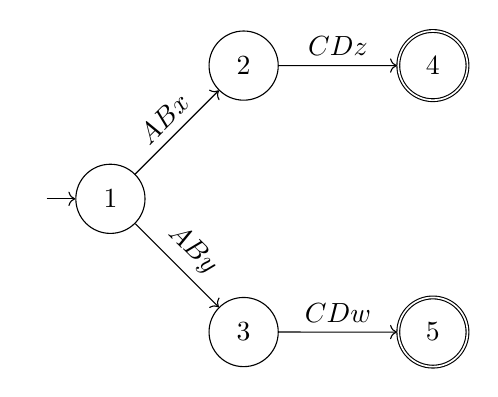
\begin{tikzpicture}[node distance=1.5cm, auto, scale=0.8]
		\node[state, initial, initial text={}] (s0) {1};
		\node[state] (s1) [above right=of s0] {2};
		\node[state] (s2) [below right=of s0] {3};
		\node[state,accepting] (s3) [right=of s1] {4};
		\node[state,accepting] (s4) [right=of s2] {5};

		\draw[->] (s0) to node[above,sloped]{$\gtlabel{A}{B}{x}$}(s1);
		\draw[->] (s0) to node[above,sloped]{$\gtlabel{A}{B}{y}$}(s2);
		\draw[->] (s1) to node[above,sloped]{$\gtlabel{C}{D}{z}$}(s3);
		\draw[->] (s2) to node[above,sloped]{$\gtlabel{C}{D}{w}$}(s4);
	\end{tikzpicture}
	\caption{An automaton representing the specification's global type given in Listing~\ref{lst:not-impl-exm}.}
	\label{fig:gt-exm}
\end{figure}
\end{example}

\bigskip

% --------------relationship between MSCs and Global Types--------------

I can now formally define the relationship between MSCs and Global Types. 
Intuitively, Global Types represent a set of MSCs, allowing us to reason 
about multiple message sequence scenarios. 

A Global Type defines a language of MSCs in two different ways, one
existential and one universal. Let $\labellanguageof{\gt}$ be the set of
sequences of arrows $w$ accepted by $\gt$. Note that for $w \in \Arrows^*$,
the function $w \mapsto \labeltomsc{w}$ with
$\labeltomsc{w} \in \mscsetofmodel{\synchmodel}$ is not injective, as two
arrows with disjoint pairs of processes commute. We write $w_1 \sim w_2$ if
$\labeltomsc{w_1} = \labeltomsc{w_2}$, and $[w]$ for the equivalence class
of $w$ with respect to $\sim$.

Informally, the existential MSC language $\existentialmsclanguageof{\gt}{}$ of a 
Global Type $\gt$ is the set of MSCs that admit at least one representation as a
sequence of arrows in $\labellanguageof{\gt}$, and the universal MSC
language $\universalmsclanguageof{\gt}$ of a Global Type $\gt$ is the set of
MSCs whose representations as sequences of arrows are all in
$\labellanguageof{\gt}$:
% TODO: ivan dice di controllare? la def di chor automata (o forse hanno una roba simile)

\bigskip

\begin{definition}[$\existentialmsclanguageof{\gt}$]
	$$
		\existentialmsclanguageof{\gt} \eqdef \{\labeltomsc{w} \mid
		w \in \labellanguageof{\gt}\}
  $$
\end{definition}

\bigskip

\begin{definition}[$\universalmsclanguageof{\gt}$]
  $$
		\universalmsclanguageof{\gt} \eqdef \{\labeltomsc{w} \mid
		[w] \subseteq \labellanguageof{\gt}\}.
	$$
\end{definition}
% TODO: dare più contesto ed esempio

\bigskip

\begin{definition}[Commutation-closed]
    A global type $\gt$ is \emph{commutation-closed} if
    $$
    \existentialmsclanguageof{\gt} = \universalmsclanguageof{\gt}.
    $$
\end{definition}
% TODO: togliere exist e forall dalla nozione
% We write $\msclanguageofcc{\gt}$ for the common language. % TODO: mi serve?

I now introduce the definition of implementability following the one given 
by Alur, et al. \cite{alur2005realizability}, referred to as 
\textit{Weak-realisability}.
To formalize it, we first define the notions of 
\textit{weak implication} and \textit{weak closure}.

%% TODO: Spiegare meglio con intuizioni

\bigskip

\begin{definition}[Weakly-imply]
	Let $\setmsc$ be a set of MSCs and $M$ an MSC. $\setmsc$
	\textit{weakly implies} $M$, if for any sequence of automata
	$\langle A_i \ |\ 1\leq i\leq n\rangle$, if every MSC in $\setmsc$ is in
	$L(\prod_i A_i)$ then $M \in L(\prod_i A_i)$.
\end{definition}

In order to understand the meaning of \emph{weak implication},
consider the following example.

\bigskip

\begin{example}
Define two MSCs, MSC1 and MSC2. Both perform the same four
communications, but in different orders.  
MSC1 first sends message $a$ from P1 to P2, then from P1 to P3, 
then sends $b$ from P4 to P2, and finally from P4 to P3.  
MSC2 instead starts with P4 sending $b$ to P2, then to P3, 
followed by P1 sending $a$ to P2 and then to P3.  

Now define a third MSC $M$ with the same four messages but in a
different order: P1 sends $a$ to P2, P4 sends $b$ to P2, P4 sends 
$b$ to P3, and finally P1 sends $a$ to P3.  

We say $M$ is weakly implied by MSC1 and MSC2. Indeed, by looking
at each process projection we recover the same behaviour in one of
them: for P1 and P4 in both, for P2 in MSC1, and for P3 in MSC2.  
Figure~\ref{fig:weak-impl} illustrates the three MSCs.

\begin{figure}[!ht]
\centering
\begin{tabular}{ccc}
\begin{minipage}{0.32\textwidth}
\scalebox{0.55}{%
\begin{msc}[left environment distance=0cm, draw frame=none, draw head=none, msc keyword=, head height=0px, label distance=0.5ex, foot height=0px, foot distance=0px]{}
	\declinst{P1}{P1}{}
	\declinst{P2}{P2}{}
	\declinst{P3}{P3}{}
	\declinst{P4}{P4}{}

	\mess{a}{P1}{P2}
	\nextlevel
	\mess[pos=0.25]{a}{P1}{P3}
	\nextlevel
	\nextlevel
	\mess[pos=0.25]{b}{P4}{P2}
	\nextlevel
	\mess{b}{P4}{P3}
\end{msc}
} 
\end{minipage}
&
\begin{minipage}{0.32\textwidth}
\scalebox{0.55}{%
\begin{msc}[left environment distance=0cm, draw frame=none, draw head=none, msc keyword=, head height=0px, label distance=0.5ex, foot height=0px, foot distance=0px]{}
	\declinst{P1}{P1}{}
	\declinst{P2}{P2}{}
	\declinst{P3}{P3}{}
	\declinst{P4}{P4}{}

	\mess[pos=0.25]{b}{P4}{P2}
	\nextlevel
	\mess{b}{P4}{P3}
	\nextlevel
	\nextlevel
	\mess{a}{P1}{P2}
	\nextlevel
	\mess[pos=0.25]{a}{P1}{P3}
\end{msc}
}
\end{minipage}
&
\begin{minipage}{0.32\textwidth}
\scalebox{0.55}{%
\begin{msc}[left environment distance=0cm, draw frame=none, draw head=none, msc keyword=, head height=0px, label distance=0.5ex, foot height=0px, foot distance=0px]{}
	\declinst{P1}{P1}{}
	\declinst{P2}{P2}{}
	\declinst{P3}{P3}{}
	\declinst{P4}{P4}{}

	\mess{a}{P1}{P2}
	\nextlevel
	\mess[pos=0.25]{b}{P4}{P2}
	\nextlevel
	\nextlevel
	\mess{b}{P4}{P3}
	\nextlevel
	\mess[pos=0.25]{a}{P1}{P3}
\end{msc}
}
\end{minipage} \\
MSC1 & MSC2 & $M$
\end{tabular}
\caption{The MSC $M$ is weakly implied by MSC1 and MSC2}
\label{fig:weak-impl}
\end{figure}
\end{example}

\bigskip

\begin{definition}[Weakly-closure $\setmsc^w$]
	The weak-closure $\setmsc^w$ of a set $\setmsc$ of MSCs contains all the MSCs
	weakly implied by $\setmsc$.
\end{definition}

% todo: esempio

\bigskip

\begin{definition}[Weakly-realisable]
	An MSC $M$ is said to be weakly-realisable if the set of MSCs
	$L(M)$ is weakly realisable. A set of MSCs $\setmsc$ is said to be weakly
	realisable if $\setmsc=\setmsc^w$.
\end{definition}
It is important to note that this definition does not include the
property of deadlock-freedom. 

% todo: esempio

% CINZIA, X TESI:
% sarebbe interessante mettere la definizione di PPDP e mostrare 
% l'equivalenza tra le due

% VERSIONE ALTERNATIVA VECCHIA
% \begin{definition}[Projection]
% For an MSC $M$ and a process $P_i$, let $M|_i$ denote the sequence of events be
% belonging to the process $P_i$ in $M$.
% \end{definition}
% \begin{definition}[Weakly-imply]
% The set of MSCs $\setmsc$ weakly implies an MSC $M$ iff for all $1\leq i\leq n$, there
% exist an MSC $M_i\in L$ such that $M|_i=M_i|_i$
% \end{definition}
% \begin{definition}[Weakly-realisable]
% ? TODO ?
% \end{definition}

We are now ready to present the main contributions of this work.


\chapter{Weak-Realisability is Undecidable for Synch Global Types}\label{sec:proof}

As already mentioned, the first contribution is Theorem~\ref{thm:main},
which states that \emph{Weak-realisability is undecidable for 
synchronous global types}. 
To understand this result, I have already covered the basic notions in 
Chapter~\ref{sec:pre} on MSCs, Global Types, and Weak-realisability. 
These concepts are general and align 
closely with definitions used in previously established works. 
We now introduce the main objects employed in the proof of Theorem~\ref{thm:main}. 
The proof itself is adapted from the work of 
Alur et~al.~\cite{alur2005realizability}. 
In between the new definition's declaration, I will also highlight the 
differences with the original proof.

\section{Definitions}
The proof is carried out by a \emph{reduction} from the
\textbf{Relaxed Post Correspondence Problem (RPCP)}, a variant of
the classical Post Correspondence Problem (PCP). 
RPCP was shown to be undecidable by
Alur~et~al.~\cite{alur2005realizability}, via reduction from PCP.
The main idea is to encode the existence of a
solution to an RPCP instance into the (non-)realisability of a
\emph{global type} (called $L^*$) built from synchronous MSCs.
Therefore, we need to prove:
$$
\Delta \in \text{RPCP} \quad\iff\quad L^* \text{ is not realisable}.
$$
In the original proof, $L^*$ is not a global type, but an MSC.
Then, we need to change some base definitions of the original paper
to fit the model. 

\bigskip

\begin{definition}[Relaxed Post Correspondence Problem]
	Given a set of tiles $\{(v_1, w_1), (v_2, w_2), ..., (v_r, w_r)\}$, 
	determine whether there exist indices $i_1, ..., i_m$ such that
	$$x_{i_1}\cdots x_{i_m} = y_{i_1}\cdots y_{i_m},$$
	where $x_{i_j}, y_{i_j} \in \{v_{i_j}, w_{i_j}\}$, such that:
	\begin{itemize}
		\item there exists at least one index $i_\ell$ for which $x_{i_\ell}\neq y_{i_\ell}$, and
		\item for all $j \leq m$, $y_{i_1}\cdots y_{i_j}$ is a prefix of $x_{i_1}\cdots x_{i_j}$.
	\end{itemize}
\end{definition}

Intuitively, RPCP requires that the concatenation on the left-hand side always 
grows at least as fast as the right-hand side, while ensuring that at least one 
chosen tile differs between the two sequences. Moreover, in constructing the 
strings, we may freely choose which element of each tile (either $v_i$ or $w_i$) 
contributes to the left or right sequence.

\bigskip

\begin{example}[Simple RPCP instance]\label{exmp:rpcp}
Consider the tile set
\[
(v_1,w_1)=(\texttt{b},\ \texttt{bb}),\quad
(v_2,w_2)=(\texttt{a},\ \texttt{ab}),\quad
(v_3,w_3)=(\texttt{c},\ \texttt{c}).
\]
Take the index sequence $(2,1,3)$ and the choices
\[
x_1 = w_2,\ y_1 = v_2;\quad
x_2 = v_1,\ y_2 = w_1;\quad
x_3 = v_3,\ y_3 = w_3.
\]
Then
\[
x_1 x_2 x_3 = \texttt{ab}\ \texttt{b}\ \texttt{c} = \texttt{abbc},
\qquad
y_1 y_2 y_3 = \texttt{a}\ \texttt{bb}\ \texttt{c} = \texttt{abbc},
\]
so the two sides are equal.

We now check the RPCP conditions:
\begin{itemize}
  \item \textbf{at least one mismatch:} here $x_1\neq y_1$ and
        $x_2\neq y_2$, so the ``some index differs'' condition holds;
  \item \textbf{prefix property:} for every prefix length $j$ we have
        $y_{1}\cdots y_{j}$ is a prefix of $x_{1}\cdots x_{j}$:
        \begin{itemize}
          \item $j=1$: $y_1=\texttt{a}$ is a prefix of $x_1=\texttt{ab}$;
          \item $j=2$: $y_1y_2=\texttt{abb}$ is a prefix of $x_1x_2=\texttt{abb}$;
          \item $j=3$: $y_1y_2y_3=\texttt{abbc}$ is a prefix of $x_1x_2x_3=\texttt{abbc}$.
        \end{itemize}
\end{itemize}
\end{example}

\bigskip

We have now identified the main problem to which our proof reduces.  
The next step is to encode an RPCP instance into an MSC.

\bigskip

\begin{definition}[$M^n_i$]\label{def:mni}
	Given the index $i$ of a tile $(v_i, w_i)$, and
	given an interger $n\in\{0,1\}$, where:
	\begin{itemize}
		\item if $n=0$, then $x_i=v_i$;
		\item if $n=1$, then $x_i=w_i$;
	\end{itemize}
	let's define the behavior of the MSC $M^n_i$.
	Firstly, Process~1 synchronously sends the message
	$m_1 = (i, n)$ to Process~2, then Process~1 transmits the index $m_2=i$
	to Process~4. Subsequently, Process~4 sends $m_3 = (i, n)$
	synchronously to Process~3. After these control messages, Process~2
	sends the characters $m_i^1 = x_i^1,..., m_i^c = x_i^c$
	synchronously to Process~3 (where $c$ is the length of $x_i$).
	This MSC is depicted in Figure~\ref{fig:mni}, 

	\begin{figure}[!ht]
		\centering
		\begin{msc}[draw frame=none, draw head=none, msc keyword=, head height=0px, label distance=0.5ex, foot height=0px, foot distance=0px]{}
			\declinst{P1}{P1}{}
			\declinst{P2}{P2}{}
			\declinst{P3}{P3}{}
			\declinst{P4}{P4}{}

			\syncmscmess{$(i,n)$}{P1}{P2}
			\syncmscmess{$i$}{P1}{P4}
			\syncmscmess{$(i,n)$}{P4}{P3}
			\syncmscmess{$x_i^1$}{P2}{P3}
			\syncmscmess{...}{P2}{P3}
			\syncmscmess{$x_i^c$}{P2}{P3}
		\end{msc}
		\caption{The $M_i^n$ MSC.}
		\label{fig:mni}
	\end{figure}

\end{definition}

Given a RPCP instance $\{(v_1,w_1),\ldots,(v_m,w_m)\}$, we associate  
with each pair $(v_i,w_i)$ two MSCs $M^0_i$ and $M^1_i$, following  
Definition~\ref{def:mni}. Each MSC $M^n_i$ is \emph{synchronous}  
(Lemma~\ref{lemma:minsynch}). Intuitively, the MSC $M_i^n$ encodes the  
construction of a string given some tiles through the interaction of four processes.  
Processes~2 and~3 are responsible for building the string itself,  
while Processes~1 and~4 transmit the index information to Processes~2  
and~3, respectively. In particular, Process~1 initiates the choice and  
forwards it to Process~4.

\bigskip

\begin{lemma}\label{lemma:minsynch}
	The MSC $M_i^n$ belongs to $\mscsetofmodel{\synchmodel}$.
\end{lemma}

\begin{proof}
	By Definition~\ref{def:linearisable-msc} and
	Definition~\ref{def:synchronous},
	we need to show a linearization with all send operations
	followed by their corresponding receive operations:
	$$
	\{~!m_1?m_1\ !m_2?m_2\ !m_3?m_3\ !m_i^1?m_i^1 \ldots !m_i^c?m_i^c~\}.
	$$
	Such a linearization exists by construction, hence $M_i^n$ is synchronous.
\end{proof}

Before establishing the connection between MSCs and  
Global Types, we briefly summarize the rationale behind the design of  
$M_i^n$.

Suppose that $\Delta=(i_1,a_1,b_1,\ldots,i_m,a_m,b_m)$ is a  
solution to the RPCP instance. From this solution we construct two MSC  
sequences:
\[
M_x = M^{a_1}_{i_1}\cdots M^{a_m}_{i_m}, \qquad  
M_y = M^{b_1}_{i_1}\cdots M^{b_m}_{i_m}.
\]
Both $M_x$ and $M_y$ are synchronous concatenations of synchronous  
MSCs. We then define a third MSC $M_{\texttt{sol}}$, obtained by  
projecting $M_y$ onto processes $P1,P2$ and $M_x$ onto processes  
$P3,P4$. Intuitively, processes $P1,P2$ represent the construction of  
the \emph{right-hand string} $y_{i_1}\cdots y_{i_m}$, while processes  
$P3,P4$ represent the construction of the \emph{left-hand string}  
$x_{i_1}\cdots x_{i_m}$. The prefix property of RPCP guarantees that  
$M_{\texttt{sol}}$ is acyclic and \emph{synchronous}. Establishing the  
synchrony of $M_{\texttt{sol}}$ is non-trivial, and this step is an  
addition to the original proof. By construction, $L^*$ weakly implies  
$M_{\texttt{sol}}$, but $M_{\texttt{sol}} \notin L^*$, since at least  
one tile differs. Consequently, $L^*$ is \emph{not realisable}.
  
With these constructions in place, we proceed to introduce the main  
objects used in the proof. Specifically, we first show how a Global  
Type can represent a single \verb|synch| MSC.

\bigskip

% TODO: ivan: forse lemma?
\begin{definition}[$G_M$]\label{def:gm}
	Given an MSC $M\in \mscsetofmodel{\synchmodel}$, there exists a
	global type $G_M$ such that $M \in \existentialmsclanguageof{\gt}$.
\end{definition}

Definition~\ref{def:gm} establishes a direct correspondence between a  
single synchronous MSC and a global type. In particular, every  
synchronous MSC can be captured precisely by a global type whose  
language contains that MSC. This correspondence will be useful  
when embedding RPCP instances into the global type framework.
We now introduce a more structured global type, parameterized by a  
string $S$, which will serve as the building block in the reduction.

\bigskip

\begin{definition}[$G_S$]\label{def:gs}
	Given a string $S\in\Sigma^*$, and two integers $i, n$,
	the global type $G_S$ is the global type composed of:
	\begin{itemize}
		\item $\mathbb{P}=\{p,q,r,s\}$;
		\item $\mathbb{M}=\{m_1,m_2,m_3,m_{S_1},...,m_{S_c}\}$ where
		      $m_1 = (i,n), m_2 = i, m_3 = (i,n),\\ m_{S_1} = S_1,...,m_{S_c} = S_c$ 
		      with $c = |S|$;
		\item Arr $=\{$\arrmess{p}{q}{m_1}, \arrmess{p}{s}{m_2}, \arrmess{s}{r}{m_3},
		      \arrmess{q}{r}{m_{S_1}}, ..., \arrmess{q}{r}{m_{S_c}}$\}$ where each arrow
		      denotes a synchronous message accompanied by an acknowledgment. % TODO: definisci/formalizza questa doppia freccia
	\end{itemize}
	$G_S$'s automaton is depicted in Figure~\ref{fig:gtype}.
	
	\begin{figure}[!ht]
		\centering
		\begin{tikzpicture}[->, node distance=35mm, on grid, auto]
			\node[state] (q0) {$q_0$};
			\node[state] (q1) [right=of q0] {$q_1$};
			\node[state] (q2) [right=of q1] {$q_2$};
			\node[state] (q3) [below left=of q0] {$q_3$};
			\node[state] (q4) [right=of q3] {$q_4$};
			\node[state] (q5) [right=of q4] {$\cdots$};
			\node[state,accepting] (q6) [right=of q5] {$q_x$};

			\path (q0) edge[] node[above] {\arrmess{p}{q}{(i,n)}} (q1);
			\path (q1) edge[] node[above] {\arrmess{p}{s}{i}} (q2);
			\path (q2) edge[] node[above left] {\arrmess{s}{r}{(i,n)}} (q3.60);
			\path (q3) edge[] node[above] {\arrmess{q}{r}{S_1}} (q4);
			\path (q4) edge[] node[above] {\arrmess{q}{r}{...}} (q5);
			\path (q5) edge[] node[above] {\arrmess{q}{r}{S_c}} (q6);
		\end{tikzpicture}
		\caption{The global type $G_S$.}
		\label{fig:gtype}
	\end{figure}

\end{definition}

Intuitively, $G_S$ specifies the same communication pattern as the MSC  
$M^n_i$ introduced in Definition~\ref{def:mni}, with the string $S$  
representing the transmitted sequence of characters. This structural  
correspondence will be made precise in the next lemma (Lemma~\ref{lmm:msgs}).  

\bigskip

% TODO: check
\begin{lemma}\label{lmm:msgs}
The MSC $M^n_i$ (Definition~\ref{def:mni}) is included in 
$\languageof{G_S}{}{}$ (Definition~\ref{def:gs}).
\end{lemma}

\begin{proof}
	Both $M^n_i$ and $G_S$ describe the same communication structure:
	process $p$ sends $(i,n)$ to $q$ and $i$ to $s$;
	process $s$ relays $(i,n)$ to $r$;
	process $q$ then sends the characters of $S$ (here matching $x_i$) to $r$.
	If $i,n$ and $S$ are the same, the sequence of messages is identical in both 
	$M^n_i$ and $G_S$. Since both models enforce synchronous communication, 
	their linearisations coincide. Hence, $M^n_i \in L(G_S)$.
\end{proof}

Having established the correspondence between an individual MSC and a  
global type, we can now extend Definition~\ref{def:gm} to encompass  
sets of MSCs, thereby capturing entire families of synchronous  
behaviours within a global type. This definition is used to easily 
construct the global type $L^*$.

\bigskip

\begin{definition}[$G^*$]\label{def:gstar}
	Given a set of MSCs $\mathcal{M} =\{M\ |\ M\in\mscsetofmodel{\synchmodel}\}$,
	$G^*$ is the set of global types such that $G^*=\{G_M\ |\ M \in \setmsc\}$,
	where $G_M$ is built using Definition~\ref{def:gm}.
\end{definition}

Informally, for every MSC $M\in\setmsc$ there exists a global type $G\in G^*$ that
captures the language of $M$. Now, let's build the automaton that represents
all the possible combinations and constructions of a set of MSCs.

\bigskip

\begin{definition}[The $L^*$ global type]\label{def:lstar}
	Assume a finite set $\setmsc$ of MSCs, where
	$\setmsc = \{M\ |\ M \in \mscsetofmodel{\synchmodel}\}$. Let $G^*$
	be defined as in Definition~\ref{def:gstar}.
	We define the global type $L^*_{N}$ as the automaton
	$\mathcal A = (Q,\Sigma, \delta, l_0, F)$ where:
	\begin{itemize}
		\item $Q = \{v_I,v_T\}\cup \bigcup_{G\in G^*} Q^G$;
		\item $\Sigma = \{\epsilon\}\cup\bigcup_{G\in G^*} \Sigma^G$;
		\item $\delta: Q \times \Sigma \rightarrow 2^Q$ is defined by:
			      \begin{enumerate}
				       \item $\forall G \in G^*,\ \delta(v_I, \varepsilon) = q_0^G$ where $q_0^G$ is the initial state of $G$,
				       \item $\forall G \in G^*,\ \forall q_f^G \in F^G,\ \delta(q_f^G, \varepsilon) = v_T$,
				       \item $\forall G, G' \in G^*,\ \forall q_f^G \in F^G,\ \delta(q_f^G, \varepsilon) = q_0^{G'}$.
			      \end{enumerate}
		\item $l_0 = v_I$ is the initial state;
		\item $F = v_T$ is the accepting state.
	\end{itemize}
	The automaton of $L^*_{N}$ is shown in Figure~\ref{fig:lstar}.  
	Finally, $L^*$ is obtained as the determinisation of $L^*_{N}$.
\end{definition}

\begin{figure}[!ht]
	\centering
	\begin{tikzpicture}[->, node distance=35mm, on grid, auto]
		\node[state] (vI) {$v_I$};
		\node[state] (qI2) [right=of vI] {$\cdots$};
		\node[state] (qI1) [above=of qI2] {$q_0^{G^1}$};
		\node[state] (qI3) [below=of qI2] {$q_0^{G^n}$};
		\node[state] (qM1) [right=of qI1] {$\cdots$};
		\node[state] (qM2) [right=of qI2] {$\cdots$};
		\node[state] (qM3) [right=of qI3] {$\cdots$};
		\node[state] (qF1) [right=of qM1] {$q_f^{G^1}$};
		\node[state] (qF2) [right=of qM2] {$\cdots$};
		\node[state] (qF3) [right=of qM3] {$q_f^{G^n}$};
		\node[state,accepting] (vT) [right=of qF2] {$v_T$};

		\path (vI) edge[] node[above] {$\epsilon$} (qI1);
		\path (vI) edge[] node[above] {$\epsilon$} (qI2);
		\path (vI) edge[] node[above] {$\epsilon$} (qI3);
		\path (qI1) edge[] node[above] {\arrmess{p}{q}{(i^{G^1},n^{G^1})}} (qM1);
		\path (qI2) edge[] node[above] {} (qM2);
		\path (qI3) edge[] node[above] {\arrmess{p}{q}{(i^{G^n},n^{G^n})}} (qM3);
		\path (qM1) edge[] node[above] {\arrmess{q}{r}{S^{G^1}_c}} (qF1);
		\path (qM2) edge[] node[above] {} (qF2);
		\path (qM3) edge[] node[above] {\arrmess{q}{r}{S^{G^n}_c}} (qF3);
		\path (qF1) edge[] node[above] {$\epsilon$} (vT);
		\path (qF2) edge[] node[above] {$\epsilon$} (vT);
		\path (qF3) edge[] node[above] {$\epsilon$} (vT);
		
		\draw (qF1.135) to [bend right=30] node[above] {$\epsilon$} (qI1.45);
		\draw (qF2.135) to [bend right=30] node[above] {$\epsilon$} (qI2.45);
		\draw (qF3.135) to [bend right=30] node[above] {$\epsilon$} (qI3.45);

		\draw (qF1.225) to node[above] {$\epsilon$} (qI2.60);
		\draw (qF3.120) to node[above] {$\epsilon$} (qI2.315);
		
		\draw (qF3) .. controls +(8,10) and +(1,3) .. node[midway,above] {$\epsilon$} (qI1);
		\draw (qF1) ..  controls +(8,-10) and +(1,-3) .. node[midway,above] {$\epsilon$} (qI3);
	\end{tikzpicture}
	\caption{The automaton of the global type $L^*_N$.}
	\label{fig:lstar}
\end{figure}

Informally, $L^*$ denotes the set of all possible executions  
arising from a family of MSCs. This construction constitutes the  
final component required for the proof, as it provides the key  
structure used to demonstrate non-realisability.

\section{Undecidability proof}

Given the definitions and lemmas state in the last section, I am now ready
to present the proof for the undecidability result.

\bigskip

\begin{theorem}\label{thm:main}
	Given a global type $G$, checking if $G$ is weakly-realisable is undecidable.
\end{theorem}

\begin{proof}
	The proof proceeds via a reduction from the RPCP problem. Let's define some useful
	elements for the proof.

	Given an instance $\Delta = \{(v_1, w_1), \ldots, (v_m, w_m)\}$ of RPCP, we
	construct a set $L$ of MSCs over four processes as follows. For each pair
	$(v_i, w_i)$, we define two MSCs, $M^0_i$ and $M^1_i$, as illustrated in
	Figure~\ref{fig:mni}.
	Observe that the communication graph of each MSC is strongly connected and
	involves all four processes. Therefore, the MSC represented from
	$L^*$ and derived from $L$ is bounded.
	With the set $L$, and following the Definition~\ref{def:lstar},
	we can construct the global type $L^*$.

	We need to prove:
	\begin{center}
		$\Delta \in \text{RPCP}$ iff the global type $L^*$ is not weakly-realisable.
	\end{center}

	\begin{itemize}
		\item[$\Rightarrow$]
		      Let's assume that
		      $\Delta = (i_1, a_1, b_1, i_2, a_2, b_2, \ldots, i_m, a_m, b_m)$ are the indices
		      for a solution to a generic RPCP problem instance, and the bits $a_j$ and
		      $b_j$ indicate which string ($v_{i_j}$ or $w_{i_j}$) is chosen to go into
		      the two (left and right)
		      long strings. Consider the new MSCs $M_x$ and $M_y$ obtained from the sequences
		      $M_x = M^{a_1}_{i_1} \cdots M^{a_m}_{i_m}$ and $M_y = M^{b_1}_{i_1} \cdots M^{b_m}_{i_m}$.
		      Executions of both of these (sequences of) MSCs must exist in any
		      realisation of $L^*$. Additionally, these MSCs are in $\mscsetofmodel{\synchmodel}$
		      because they are sequence of $\mscsetofmodel{\synchmodel}$ MSC (Lemma~\ref{lemma:minsynch}).
		      $M_x$ corresponds to the construction of the left side of the equivalence of the RPCP
		      problem, and, instead, $M_y$ represents the construction of the right side.
		      We then look at the projections $M_x|_1$, $M_x|_2$, $M_x|_3$,
		      and $M_x|_4$ of $M_x$, and $M_y|_1$, $M_y|_2$, $M_y|_3$, $M_y|_4$ of $M_y$ onto the
		      4 processes. Now consider an MSC $M_{\texttt{sol}}$ formed from $M_y|_1$, $M_y|_2$,
		      $M_x|_3$, and $M_x|_4$. This MSC represent the construction of the solution to
		      the problem. Processes 1 and 2 construct the right part ($y_{i_1}...y_{i_m}$)
		      and processes 3 and 4 construct the left part ($x_{i_1}...x_{i_m}$).
		      The claim is that the combined MSC $M_{\texttt{sol}}$ is weakly
		      implied by $L^*$. By definition, the only thing to establish is that $M_{\texttt{sol}}$
		      is indeed an MSC, in the sense that it is acyclic, well-formed, complete
		      and synchronous.
		      The only new situation in terms of communication in $M_{\texttt{sol}}$ is the
		      communication between $P_1$ and $P_4$, and between $P_2$ and $P_3$.
		      But the communication between $P_1$ and $P_4$ is consistent in
		      $M_y|_1$ and $M_x|_4$ (i.e., the sequence of messages sent from $P_1$ to
		      $P_4$ in $M_y|_1$ is equal to the sequence of messages received in $M_x|_4$),
		      and the communication between $P_2$ and $P_3$ is consistent in
		      $M_y|_2$ and $M_x|_3$ because $R$ is a solution to the RPCP.
		      Furthermore, the acyclicity of $M_{\texttt{sol}}$ follows from the property of the
		      solution that the string formed by the first $j$ words on processes 1
		      and 2 is always a prefix of the string formed by the first $j$ words
		      on processes 3 and 4. Consequently, each message from $P_1$ to $P_4$
		      is sent before it needs to be received.

		      Finally, we prove that $M_{\texttt{sol}} \in \mscsetofmodel{\synchmodel}$.
		      Assume, for contradiction, that $M_{\texttt{sol}} \notin \mscsetofmodel{\synchmodel}$.
		      Then, there should be a cycle of dependencies in the communication pattern.
		      There are no communication between $P_2$ and $P_4$, and between $P_1$
		      and $P_3$. Therefore, this cycle must involve all processes, starting
		      for example from $P_1$ and having this dependency graph
		      $P_1\leftrightarrow P_2\leftrightarrow P_3\leftrightarrow P_4\leftrightarrow P_1$.
		      The only new situation that we now that can cause a cycle are the communication
		      between $P_1$ and $P_4$, and between $P_2$ and $P_3$.
		      We don't need to analyse the new communication between $P_1$ and $P_4$ because
		      it's not feasible in any communication model, but we need to analyse the one
		      between $P_2$ and $P_3$ because it's feasible in FIFO.

		      % For the fist comunication, the only possible cycle pattern is depicted
		      % in Fig.~\ref{fig:cycle1}

		      % \begin{figure}[!ht]
		      %  \centering
		      %  \begin{msc}[draw frame=none, draw head=none, msc keyword=, head height=0px, label distance=0.5ex, foot height=0px, foot distance=0px]{}
		      %   \declinst{P1}{P1}{}
		      %   \declinst{P2}{P2}{}
		      %   \declinst{P3}{P3}{}
		      %   \declinst{P4}{P4}{}

		      %   \mess[label position=above right,pos=0.45]{$i_z$}{P1}{P4}[8]
		      %   \nextlevel
		      %   \nextlevel
		      %   \nextlevel
		      %   \syncmscmess{($i_k,n_k)$}{P1}{P2}
		      %   \mess[label position=above,pos=0.62]{$i_k$}{P1}{P4}
		      %   \mess{}{P4}{P1}
		      %   \nextlevel
		      %   \syncmscmess{$(i_k,n_j)$}{P3}{P4}
		      %   \nextlevel
		      %   \nextlevel
		      %   \mess{}{P4}{P1}[-8]
		      %  \end{msc}
		      %  \caption{The $M_i^n$ MSC.}
		      %  \label{fig:cycle1}
		      % \end{figure}

		      % This cycle is not possible because it does not represent a
		      % solution to the RPCP problem:
		      % $x_1...x_{i_k}...x_{i_z}...x_m \neq y_1...y_{i_z}...y_{i_k}...y_m$.

		      \begin{figure}[!ht]
			      \centering
			      \begin{msc}[draw frame=none, draw head=none, msc keyword=, head height=0px, label distance=0.5ex, foot height=0px, foot distance=0px]{}
				      \declinst{P1}{P1}{}
				      \declinst{P2}{P2}{}
				      \declinst{P3}{P3}{}
				      \declinst{P4}{P4}{}

				      \mess[label position=above right, pos=0.3]{$c$}{P2}{P3}[4]%
				      \nextlevel
				      \syncmscmess{$(i_k,n_k)$}{P1}{P2}
				      \mess[pos=0.62]{$i_k$}{P1}{P4}%
				      \mess{}{P4}{P1}
				      \nextlevel
				      \syncmscmess{$(i_k,n_j)$}{P3}{P4}
				      \mess{}{P3}{P2}[-4]
			      \end{msc}
			      \caption{MSC communication that breaks synchrony.} % todo: modifica
			      \label{fig:cycle2}
		      \end{figure}

		      For the communication between $P_2$ and $P_3$, the only possible cycle
		      pattern is depicted in Fig.~\ref{fig:cycle2}.
		      Suppose $P_2$ wants to send a character $c$, but $P_3$
		      is not expecting any further characters. In order for
		      $P_3$ to resume receiving, it must first receive an index
		      from $P_4$. However, $P_4$ can only send this index
		      after receiving it from $P_1$, which in turn must first
		      communicate the index to $P_2$.
		      At this point, $P_2$ needs to receive the index from
		      $P_1$, but it cannot do so until it finishes sending
		      character $c$. This creates a circular dependency among the
		      processes, making the communication pattern impossible. % TODO: chiarire che non è come un caso di deadlock
		      This cycle would break the prefix property as
		      $x_1...x_{k-1}...x_m= y_1...y_{k-1}...y_m$, but the character $c$ appears
		      in $y_1...y_{k-1}$ but not in $x_1...y_{k-1}$ contradicting the
		      assumption that $y_1...y_{k-1} \leq x_1...x_{k-1}$.
		      Therefore, we conclude that $M_{\texttt{sol}} \in \mscsetofmodel{\synchmodel}$.

		      Note that $M_{\texttt{sol}}$ cannot itself be in $L^*$ because there must be
		      some index $i_j$ where $a_j \neq b_j$, and no MSC exists in $L$ where,
		      after $P_1$ announces the index, what $P_2$ sends is not
		      identical to what $P_3$ receives.

		\item[$\Leftarrow$]
		      Suppose there is some MSC $M^@$ which
		      exists in any realisation of $L^*$, but is not in $L^*$ itself. We want
		      to derive a solution to $\Delta$ from $M^@$.
		      First, it is clear that the projection $M^@|_1$ must consist of a sequence
		      of pairs of messages (the first of each pair acknowledged), sent from
		      process 1 to processes 2 and 4, respectively, with messages $(i, b)$ and $i$.
		      Likewise, it is clear that, in order for process 2 to receive those messages,
		      $M^@|_2$ must consist of a sequence of receipts of $(i, b)$ pairs, and after
		      each $(i, b)$, either $v_i$ or $w_i$ is sent to process 3, based on whether
		      $b = 0$ or $b = 1$, before the next index pair is received.
		      Likewise, $M^@|_4$ consists of a sequence of receipts of index $i$ from
		      process 1, followed by sending of $(i, 0)$ or $(i, 1)$ to process 3, and
		      $M^@|_3$ consists of a sequence of receipt of $(i, 0)$ or $(i, 1)$ followed
		      by receipt of $v_i$ or $w_i$, respectively.
		      Now, since $M^@$ is not in $L^*$, for some index $i$ the choice of $v_i$ or
		      $w_i$ must differ on process 2 and process 3. (Note, we are assuming that
		      the buffers between processes are FIFO.)
		      Furthermore, because of the precedences, the prefix formed by the first
		      $j$ words on process 2 must precede the $(j + 1)$-th message from
		      process 1 to process 4, which in turn precedes the $(j + 1)$-th message
		      from 4 to 3, and hence the $(j + 1)$-th word on process 3. That is, the
		      string formed by the first $j$ words on process 2 is a prefix of the string
		      formed by the first $j$ words on process 3. Therefore, we can readily
		      build a solution for $\Delta$ from $M^@$ by building the strings of the solution
		      taking the projections of $P_1$ and $P_4$. In fact, $P_1$ builds 
			  $y_{i_1}\cdots y_{i_m},$ and $P_4$ builds $x_{i_1}\cdots x_{i_m}$.

	\end{itemize}

\end{proof}

In this example, I will show the step-by-step construction 
of $M_{\texttt{sol}}$ from Theorem~\ref{thm:main}.

\bigskip

% TODO: dare un esempietto per far vedere che la prova regge
% Andrà bene?
\begin{example}[$M_{\texttt{sol}}$ Example of Theorem~\ref{thm:main}]
Consider the tiles and the solution of the RPCP instance 
in Example~\ref{exmp:rpcp}, with the tile set and the solution
with index sequence $(2,1,3)$
$$
 (v_1,w_1)=(\texttt{b},\texttt{bb}),\ 
 (v_2,w_2)=(\texttt{a},\texttt{ab}),\ 
 (v_3,w_3)=(\texttt{c},\texttt{c}).
$$
$$
 x_1=w_2,\ y_1=v_2;\quad x_2=v_1,\ y_2=w_1;\quad x_3=v_3,\ y_3=w_3
$$
This sequence is a solution because
$x_1x_2x_3=\texttt{ab}\,\texttt{b}\,\texttt{c}=\texttt{abbc}$ and
$y_1y_2y_3=\texttt{a}\,\texttt{bb}\,\texttt{c}=\texttt{abbc}$. The
prefix property and the ``some index differs'' condition are satisfied.

Therefore, the encoding of the solution is
$$\Delta = (i_1=2,a_1=1,b_1=0,i_2=1,a_2=0,b_2=1,i_3=3,a_3=0,b_3=1)$$

Recall that for each tile index \(i\) we have two synchronous MSCs
\(M_i^0\) and \(M_i^1\) (see Definition~\ref{def:mni}), where the bit
indicates choosing \(v_i\) (0) or \(w_i\) (1) for the character stream.
Using the concrete index sequence \((2,1,3)\) we form two
concatenated MSCs:
\[
  M_x\;=\; M^{1}_{2}\ \cdot\ M^{0}_{1}\ \cdot\ M^{0}_{3},
\qquad
  M_y\;=\; M^{0}_{2}\ \cdot\ M^{1}_{1}\ \cdot\ M^{1}_{3}.
\]
Here \(M\) encodes the \(\mathbf{x}\)-concatenation
\((x_1,x_2,x_3)=(w_2,v_1,v_3)\) (depicted 
in Figure~\ref{fig:exmp-mx}) and \(M_y\) encodes 
the \(\mathbf{y}\)-concatenation (depicted in 
Figure~\ref{fig:exmp-my}) \((y_1,y_2,y_3)=(v_2,w_1,w_3)\).

\begin{figure}[!ht]
\centering
\begin{msc}[draw frame=none, draw head=none, msc keyword=, head height=0px, label distance=0.5ex, foot height=0px, foot distance=0px]{}
	\declinst{P1}{P1}{}
	\declinst{P2}{P2}{}
	\declinst{P3}{P3}{}
	\declinst{P4}{P4}{}

	\syncmscmess{$(2,1)$}{P1}{P2}
	\syncmscmess{$2$}{P1}{P4}
	\syncmscmess{$(2,1)$}{P4}{P3}
	\syncmscmess{$a$}{P2}{P3}
	\syncmscmess{$b$}{P2}{P3}

	\syncmscmess{$(1,0)$}{P1}{P2}
	\syncmscmess{$1$}{P1}{P4}
	\syncmscmess{$(1,0)$}{P4}{P3}
	\syncmscmess{$b$}{P2}{P3}

	\syncmscmess{$(3,0)$}{P1}{P2}
	\syncmscmess{$3$}{P1}{P4}
	\syncmscmess{$(3,0)$}{P4}{P3}
	\syncmscmess{$c$}{P2}{P3}
\end{msc}
\caption{The MSC $M_x$}
\label{fig:exmp-mx}
\end{figure}

\begin{figure}[!ht]
\centering
\begin{msc}[draw frame=none, draw head=none, msc keyword=, head height=0px, label distance=0.5ex, foot height=0px, foot distance=0px]{}
	\declinst{P1}{P1}{}
	\declinst{P2}{P2}{}
	\declinst{P3}{P3}{}
	\declinst{P4}{P4}{}

	\syncmscmess{$(2,0)$}{P1}{P2}
	\syncmscmess{$2$}{P1}{P4}
	\syncmscmess{$(2,0)$}{P4}{P3}
	\syncmscmess{$a$}{P2}{P3}

	\syncmscmess{$(1,1)$}{P1}{P2}
	\syncmscmess{$1$}{P1}{P4}
	\syncmscmess{$(1,1)$}{P4}{P3}
	\syncmscmess{$b$}{P2}{P3}
	\syncmscmess{$b$}{P2}{P3}

	\syncmscmess{$(3,1)$}{P1}{P2}
	\syncmscmess{$3$}{P1}{P4}
	\syncmscmess{$(3,1)$}{P4}{P3}
	\syncmscmess{$c$}{P2}{P3}
\end{msc}
\caption{The MSC $M_y$}
\label{fig:exmp-my}
\end{figure}

Recall that $M|_p$ denote the projection of $M$ onto process $p$. We
construct the MSC
$$
  M_{\texttt{sol}} = (M_y|_{P1},\; M_y|_{P2},\; M_x|_{P3},\; M_x|_{P4}),
$$
i.e.\ processes $1,2$ follow $M_y$ while $3,4$ follow $M_x$.
Intuitively, $M_{\texttt{sol}}$ pairs the right-side construction (from $M_y$)
with the left-side construction (from $M_x$). 
Figure~\ref{fig:exmp-msol} illustrates the behaviour of the MSC
$M_{\texttt{sol}}$. Observe that when process~3 expects to receive the
second character $\texttt{b}$ right after $a$, 
but process~2 cannot send it immediately:
it must first obtain the corresponding index and bit from process~1.
The prefix property guarantees
that every partial construction of the right-hand side is aligned with
a prefix of the left-hand side, therefore preserving synchronous
semantics throughout the execution.

\begin{figure}[!ht]
\centering
\begin{msc}[draw frame=none, draw head=none, msc keyword=, head height=0px, label distance=0.5ex, foot height=0px, foot distance=0px]{}
	\declinst{P1}{}{$M_y|_{P1}$}
	\declinst{P2}{}{$M_y|_{P2}$}
	\declinst{P3}{}{$M_x|_{P3}$}
	\declinst{P4}{}{$M_x|_{P4}$}

	\syncmscmess{$(2,1)$}{P1}{P2}
	\syncmscmess{$2$}{P1}{P4}
	\syncmscmess{$(2,0)$}{P4}{P3}
	\syncmscmess{$a$}{P2}{P3}
	\mess{}{P3}{P2}[4]
	\nextlevel

	\syncmscmess{$(1,0)$}{P1}{P2}
	\mess[pos=0.4]{$1$}{P1}{P4}
	\mess{}{P4}{P1}
	\nextlevel
	\syncmscmess{$(1,1)$}{P4}{P3}
	\mess[pos=0.2]{$b$}{P2}{P3}[-4]
	\nextlevel
	\syncmscmess{$b$}{P2}{P3}
	
	\syncmscmess{$(3,0)$}{P1}{P2}
	\syncmscmess{$3$}{P1}{P4}
	\syncmscmess{$(3,1)$}{P4}{P3}
	\syncmscmess{$c$}{P2}{P3}
\end{msc}
\caption{The MSC $M_\texttt{sol}$}
\label{fig:exmp-msol}
\end{figure}

\end{example}

The sequence of lemmas and the main theorem collectively establish the
undecidability of weak-realisability for global types. Having developed the
theoretical foundation, we now move to the next section, where we focus on the
practical aspects of analysing realisability, and introduce the \textsc{ReSCu} tool.

\chapter{ReSCu}\label{sec:rescu}
I now present \textsc{ReSCu} (first introduced in \cite{desgeorges2023rsc, di2023multiparty, guizouarn2023communicating}),
describing its features, the input
language it uses, its implementation, and the modifications I introduced to
extend its functionality~\cite{rescuoriginalrepo}. The updated repository with 
the new examples is available on GitHub~\cite{rescurepo}.

\section{Characteristics}
\textsc{ReSCu} is a command-line tool that can check both membership in the 
class of \verb|synch| systems (called Realizable with Synchronous Communication 
or, in brief, RSC from now on) and reachability of regular sets of configurations. It 
accepts input systems with arbitrary topologies and supports both FIFO and 
bag buffers. The tool provides several options: 
\verb|-isrsc| checks whether the system is RSC, and \verb|-mc| checks reachability of 
bad configurations. Both checks can be combined in a single run. The \verb|-fifo| option 
overrides buffer types by treating all as FIFO. When a system is unsafe, the 
\verb|-counter| option (used with \verb|-mc|) produces an RSC execution that leads 
to the bad configuration, while the same option used with \verb|-isrsc| outputs the 
borderline violation execution if the system is not RSC. Additional features include 
a progress display to estimate remaining runtime during long computations, and 
\verb|-to_dot|, which exports the system to DOT format for visualization.
One of the most similar tools is \textsc{McScm} \cite{heussner2012mcscm}, that
uses a framework with for different verification techniques. 
Symbolic Communicating Machines (SCM), defined and used in \cite{brand1983communicating} 
serve as the input format of the tool.
The grammar has been updated to provide greater flexibility and clarity. In
particular, transition guards have been made optional (with a default value
\verb|: when true|), and a new \verb|final| keyword has been introduced to
explicitly specify final states. The updated grammar is shown in
Listing~\ref{lst:scm-grammar}. 
A formal definition for this object is stated
in Definition~\ref{def:cfsm}.

\begin{lstlisting}[language={},caption={Simplified SCM grammar},
    keywordstyle=\color{blue}\bfseries,label={lst:scm-grammar}] 
prog         ::= <header> <aut_list> [<bad_confs>]
header       ::= scm <ident>:<channels> [<bags>] <parameters>
channels     ::= nb_channels = <int>;
bags         ::= //# bag_buffers = <int_list>
int_list     ::= <int>
               | <int_list>, <int>
parameters   ::= parameters = <param_list>
param_list   ::= <param>
               | <param> <param_list>
param        ::= {int | real} <ident>;
aut_list     ::= automaton <ident>:<initial>;<final>; <state_list>
initial      ::= initial : <int_list>;
final        ::= final : <int_list>;
state_list   ::= <state>
               | <state_list> <state>
state        ::= state <int> : <trans_list>
trans_list   ::= <transition>
               | <trans_list> <transition>
guard        ::= : when true | <nothing>
transition   ::= to <int> : when true , <int> <action> <ident>
action       ::= "!" | "?"
bad_confs    ::= bad_states: <bad_list>
bad_list     ::= (<bad_conf>)
               | <bad_list> (<bad_conf>)
bad_conf     ::= <bad_state>
               | <bad_state> with <bad_buffers>
bad_state    ::= automaton <ident>: in <int>: true [<bad_state>]
bad_buffers  ::= <regular_expression>
nothing      ::= 
\end{lstlisting}

\section{Progress and Deadlock-Freedom}
I extended \textsc{ReSCu} with verification routines that focus on two
fundamental correctness properties of distributed systems: \emph{progress} and
\emph{deadlock-freedom}. To enable this, the tool constructs the synchronous
system using the synchronous product whenever the input SCM is recognized as an
RSC. These two verification routines are triggered only after another check: 
once the system is proven to be RSC, we can safely construct a well-formed 
synchronous product from it. We consider the definitions given in Chapter~\ref{sec:pre}.
Definition~\eqref{def:cfsm} corresponds to the concept of an SCM. We now present the
definition of the Synchronous Product for CFSMs, which has been implemented in the
tool and serves as a key component for analyzing.

\begin{definition}[Synchronous Product]
Let $\mathcal{S} = (\mathcal{A}_p)_{p \in \mathbb{P}}$ be a system of CFSMs, where 
$\mathcal{A}_p = (L_p, \mathit{Act}_p, \delta_p, l_{0,p}, F_p)$ is the CFSM associated 
to process $p$.  

The \emph{synchronous product} of $\mathcal{S}$ is the global type 
$\mathrm{prod}(\mathcal{S}) = (L, \mathit{Arr}, \delta, l_0, F)$,
where
\begin{itemize}
    \item $L = \prod_{p \in \mathbb{P}} L_p$ is the set of global locations,
    \item $l_0 = (l_{0,p})_{p \in \mathbb{P}}$ is the initial global state,
    \item $F = \prod_{p \in \mathbb{P}} F_p$ is the set of global final states,
    \item $\delta$ is the transition relation defined as follows:  
    $(\vec{l}, \; p \xrightarrow{m} q, \; \vec{l}\,') \in \delta$ if
    \[
    (l_p,\, !m^{p \to q},\, l'_p) \in \delta_p, \quad 
    (l_q,\, ?m^{p \to q},\, l'_q) \in \delta_q, \quad 
    l'_r = l_r \;\; \text{for all } r \notin \{p,q\}.
    \]
\end{itemize}
\end{definition}

After constructing the synchronous product, the tool performs several
important post-processing operations. In particular, it removes any
unreachable nodes from the resulting product, simplifying the structure
and ensuring that only relevant states are retained for further analysis.
We can now define the two properties added to the tool.

I denote $\text{Reach}$ as the function that, given a node, gives the set of 
reachable nodes, and $\text{Init}, \text{Final}$ as the initial and final node.
Informally, a given system satisfies \emph{progress} if, 
from every reachable node,
either the system can eventually perform a transition, or the node is
a final one.
\begin{definition}[Progress]
	A system $S$ has the progress property iff $\text{Prod}_{sync}(S)$
	has the property
	$\text{Reach}(\text{Init})\subseteq \text{Reach}(\text{Final})$.
\end{definition}

%% sostituire posit con reach: sono tutti gli stati raggiungibili

In other words, this property is implemented by checking for all nodes 
that are not a final state
if they are without any outgoing transitions. 
This definition allows infinite loops.
Informally, a system is \emph{deadlock-free} if no reachable
non-final node exists in which all processes are blocked (i.e., no further
actions can be taken).

\begin{definition}[Deadlock-Freedom]
	A system $S$ is deadlock-free iff
    $\text{Prod}_{\text{sync}}(S)$ has the property
	$\text{Reach}(\text{Init})\subseteq \text{Prefixes}(\text{Final})$.
\end{definition}
%% mettere controesempio x questa def: in un sistema non sincrono potrei non vedere un deadlock con questa def

%% nella tesi mettere la def di ppdp spiegata bene che è quella che include tutte le semantiche di network

% Intuitively, the set of all the execution that starts from the initial state
% are a section of the set of all prefixes of the executions that start from
% the final state.
More precisely, a system that can reach, from its initial states, some state
that does not lead to a final state is not deadlock-free. Under this definition,
even a loop that never reaches a final state is considered a deadlock,
making the property more restrictive. This check is implemented using a
reverse search algorithm starting from the final states.

Additionally, the synchronized system can be exported in DOT format
(with a default filename of \verb|sync.dot|), which allows for graphical 
visualization of its structure and behavior.
% Some illustrative examples 
% demonstrating these new features are included in the
% \verb|rescu/examples/deadlock| folder.
Let's finally see some relevant examples.

% CINZIA, X TESI:
% pensare ad un esempio che fa vedere che non è vero in generale

\section{Examples}

To illustrate these notions, I present two examples. The first is the
classical \emph{Dining Philosophers} problem, which shows how resource
contention can lead to deadlock. The second is a minimal looping system
that demonstrates how a process may satisfy the progress property while
still failing to be deadlock-free.

\begin{example}\label{exm:philo}
Consider two philosophers $P_0, P_1$ and two forks $F_1, F_2$, arranged
so that each philosopher needs both forks to eat. If both philosophers
pick up their left fork simultaneously, each waits indefinitely for the
other fork, producing a deadlock. This captures the essence of the Dining
Philosophers problem: concurrent processes blocking one another when
competing for shared resources.

\begin{lstlisting}[language={},caption={Output of Example~\ref{exm:philo}},
    label={lst:philo}]
This system is RSC.
There are some sink states:
Sink: Id=11 Configuration={{ F0:4; F1:3; P1:2; P2:2 }}
There are some deadlock states:
Deadlock: Id=4 Configuration={{ F0:2; F1:1; P1:1; P2:1 }}
Deadlock: Id=11 Configuration={{ F0:4; F1:3; P1:2; P2:2 }}
Deadlock: Id=8 Configuration={{ F0:4; F1:1; P1:1; P2:2 }}
Deadlock: Id=7 Configuration={{ F0:2; F1:3; P1:2; P2:1 }}
\end{lstlisting}

The behavior of the four participants is shown in
Figure~\ref{fig:philo}. Running the tool on
this input produces the terminal output in
Listing~\ref{lst:philo} and the corresponding synchronous system in
Figure~\ref{fig:philo-sync}. In the
generated figure, the red state marks a configuration where no further
actions are possible, while the three yellow states correspond to
deadlocks, i.e.\ executions where both philosophers wait for each other
indefinitely. The terminal output also lists the precise configurations
of these problematic states.

\newpage

\begin{figure}[!ht]
    \centering
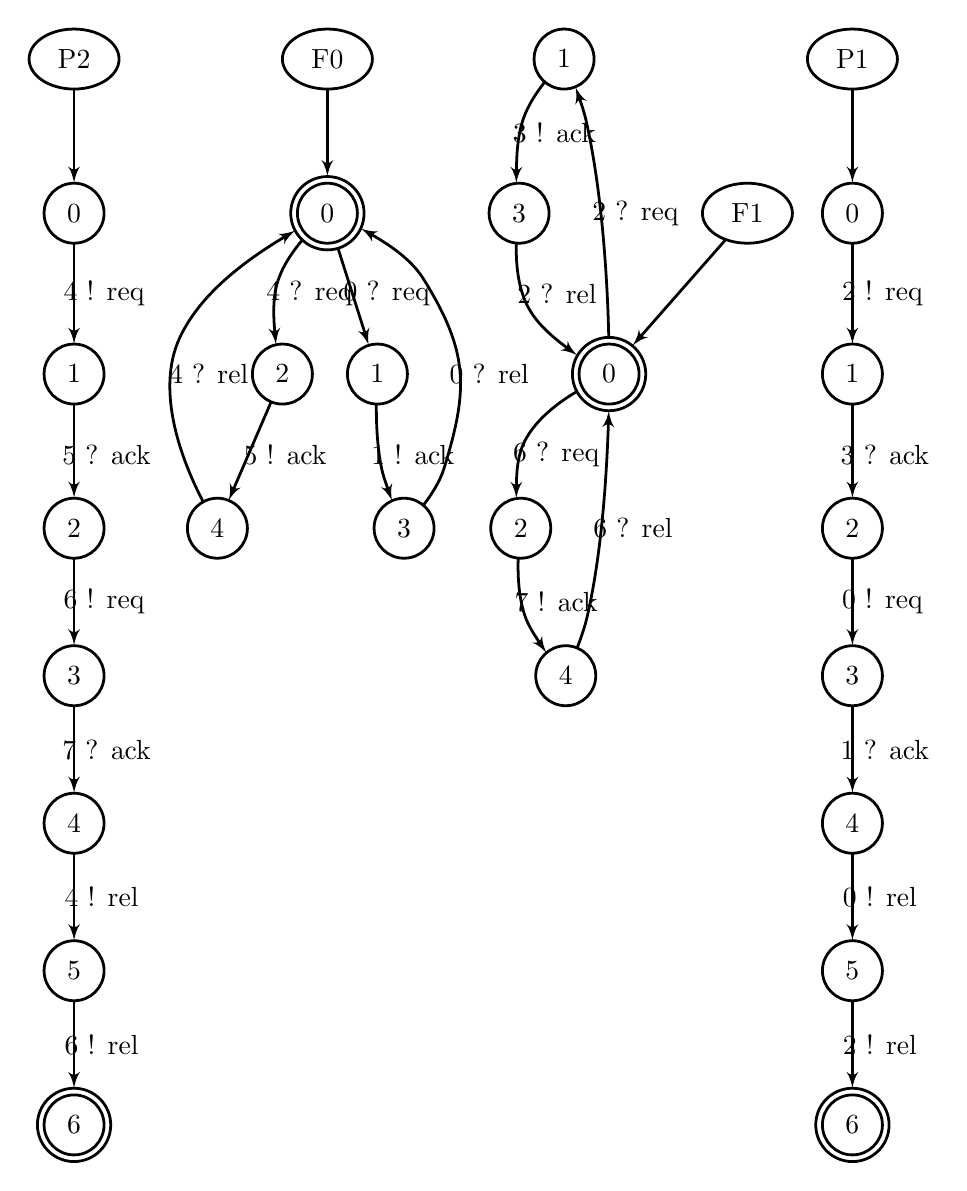
\begin{tikzpicture}[>=latex',line join=bevel,scale=0.6]
  \pgfsetlinewidth{1bp}
%%
\pgfsetcolor{black}
  % Edge: P23 -> P24
  \draw [->] (27.0bp,273.41bp) .. controls (27.0bp,261.76bp) and (27.0bp,246.05bp)  .. (27.0bp,221.35bp);
  \definecolor{strokecol}{rgb}{0.0,0.0,0.0};
  \pgfsetstrokecolor{strokecol}
  \draw (46.5bp,247.25bp) node {7 ? ack};
  % Edge: F00 -> F02
  \draw [->] (163.75bp,552.68bp) .. controls (158.12bp,545.99bp) and (152.42bp,537.69bp)  .. (149.5bp,529.0bp) .. controls (146.63bp,520.45bp) and (146.19bp,510.74bp)  .. (148.12bp,490.45bp);
  \draw (168.25bp,520.75bp) node {4 ? req};
  % Edge: F00 -> F01
  \draw [->] (185.51bp,547.49bp) .. controls (189.85bp,533.83bp) and (195.6bp,515.7bp)  .. (203.7bp,490.19bp);
  \draw (214.55bp,520.75bp) node {0 ? req};
  % Edge: F11 -> F13
  \draw [->] (309.26bp,647.53bp) .. controls (304.38bp,641.32bp) and (299.22bp,633.51bp)  .. (296.5bp,625.5bp) .. controls (293.62bp,617.02bp) and (292.5bp,607.4bp)  .. (292.34bp,587.21bp);
  \draw (315.25bp,617.25bp) node {3 ! ack};
  % Edge: F02 -> F04
  \draw [->] (145.21bp,455.74bp) .. controls (139.43bp,442.32bp) and (131.01bp,422.79bp)  .. (119.85bp,396.89bp);
  \draw (153.59bp,424.25bp) node {5 ! ack};
  % Edge: P21 -> P22
  \draw [->] (27.0bp,454.05bp) .. controls (27.0bp,441.53bp) and (27.0bp,424.37bp)  .. (27.0bp,398.4bp);
  \draw (46.5bp,424.25bp) node {5 ? ack};
  % Edge: P1dummy -> P10
  \draw [->] (494.0bp,643.9bp) .. controls (494.0bp,631.26bp) and (494.0bp,613.55bp)  .. (494.0bp,587.42bp);
  % Edge: F10 -> F11
  \draw [->] (347.8bp,494.92bp) .. controls (347.12bp,524.61bp) and (344.41bp,579.76bp)  .. (334.0bp,625.5bp) .. controls (333.39bp,628.17bp) and (332.63bp,630.9bp)  .. (328.0bp,644.39bp);
  \draw (363.84bp,569.0bp) node {2 ? req};
  % Edge: F10 -> F12
  \draw [->] (328.44bp,461.89bp) .. controls (317.28bp,455.28bp) and (304.21bp,445.37bp)  .. (297.5bp,432.5bp) .. controls (293.87bp,425.54bp) and (292.43bp,417.31bp)  .. (292.34bp,398.17bp);
  \draw (316.25bp,424.25bp) node {6 ? req};
  % Edge: P15 -> P16
  \draw [->] (494.0bp,96.051bp) .. controls (494.0bp,84.609bp) and (494.0bp,69.297bp)  .. (494.0bp,44.218bp);
  \draw (510.5bp,70.25bp) node {2 ! rel};
  % Edge: F14 -> F10
  \draw [->] (329.0bp,308.61bp) .. controls (331.27bp,314.45bp) and (333.57bp,321.18bp)  .. (335.0bp,327.5bp) .. controls (343.53bp,365.15bp) and (346.5bp,409.54bp)  .. (347.83bp,450.24bp);
  \draw (362.3bp,380.0bp) node {6 ? rel};
  % Edge: P11 -> P12
  \draw [->] (494.0bp,454.05bp) .. controls (494.0bp,441.53bp) and (494.0bp,424.37bp)  .. (494.0bp,398.4bp);
  \draw (513.5bp,424.25bp) node {3 ? ack};
  % Edge: P10 -> P11
  \draw [->] (494.0bp,550.67bp) .. controls (494.0bp,537.08bp) and (494.0bp,517.89bp)  .. (494.0bp,490.72bp);
  \draw (512.0bp,520.75bp) node {2 ! req};
  % Edge: P12 -> P13
  \draw [->] (494.0bp,361.91bp) .. controls (494.0bp,350.26bp) and (494.0bp,334.55bp)  .. (494.0bp,309.85bp);
  \draw (512.0bp,335.75bp) node {0 ! req};
  % Edge: F12 -> F14
  \draw [->] (293.48bp,361.86bp) .. controls (293.15bp,351.62bp) and (293.73bp,338.51bp)  .. (297.5bp,327.5bp) .. controls (299.0bp,323.12bp) and (301.22bp,318.8bp)  .. (310.27bp,305.48bp);
  \draw (316.25bp,335.75bp) node {7 ! ack};
  % Edge: F1dummy -> F10
  \draw [->] (418.03bp,553.23bp) .. controls (405.14bp,538.56bp) and (385.13bp,515.78bp)  .. (362.27bp,489.75bp);
  % Edge: P13 -> P14
  \draw [->] (494.0bp,273.41bp) .. controls (494.0bp,261.76bp) and (494.0bp,246.05bp)  .. (494.0bp,221.35bp);
  \draw (513.5bp,247.25bp) node {1 ? ack};
  % Edge: F04 -> F00
  \draw [->] (104.36bp,396.04bp) .. controls (92.695bp,418.48bp) and (75.05bp,461.59bp)  .. (90.5bp,494.5bp) .. controls (102.62bp,520.33bp) and (128.78bp,540.22bp)  .. (159.49bp,558.47bp);
  \draw (107.75bp,472.5bp) node {4 ? rel};
  % Edge: P24 -> P25
  \draw [->] (27.0bp,184.91bp) .. controls (27.0bp,173.26bp) and (27.0bp,157.55bp)  .. (27.0bp,132.85bp);
  \draw (43.5bp,158.75bp) node {4 ! rel};
  % Edge: F01 -> F03
  \draw [->] (208.36bp,454.32bp) .. controls (208.29bp,443.26bp) and (208.85bp,428.65bp)  .. (211.5bp,416.0bp) .. controls (212.1bp,413.16bp) and (212.89bp,410.24bp)  .. (217.7bp,396.7bp);
  \draw (230.25bp,424.25bp) node {1 ! ack};
  % Edge: F03 -> F00
  \draw [->] (236.67bp,393.95bp) .. controls (241.48bp,400.16bp) and (246.51bp,407.98bp)  .. (249.0bp,416.0bp) .. controls (263.95bp,464.24bp) and (263.45bp,485.98bp)  .. (237.0bp,529.0bp) .. controls (230.4bp,539.73bp) and (219.62bp,548.17bp)  .. (199.3bp,559.73bp);
  \draw (276.13bp,472.5bp) node {0 ? rel};
  % Edge: P14 -> P15
  \draw [->] (494.0bp,184.91bp) .. controls (494.0bp,173.26bp) and (494.0bp,157.55bp)  .. (494.0bp,132.85bp);
  \draw (510.5bp,158.75bp) node {0 ! rel};
  % Edge: P2dummy -> P20
  \draw [->] (27.0bp,643.9bp) .. controls (27.0bp,631.26bp) and (27.0bp,613.55bp)  .. (27.0bp,587.42bp);
  % Edge: P25 -> P26
  \draw [->] (27.0bp,96.051bp) .. controls (27.0bp,84.609bp) and (27.0bp,69.297bp)  .. (27.0bp,44.218bp);
  \draw (43.5bp,70.25bp) node {6 ! rel};
  % Edge: P20 -> P21
  \draw [->] (27.0bp,550.67bp) .. controls (27.0bp,537.08bp) and (27.0bp,517.89bp)  .. (27.0bp,490.72bp);
  \draw (45.0bp,520.75bp) node {4 ! req};
  % Edge: F0dummy -> F00
  \draw [->] (179.0bp,643.9bp) .. controls (179.0bp,632.34bp) and (179.0bp,616.54bp)  .. (179.0bp,591.29bp);
  % Edge: F13 -> F10
  \draw [->] (292.37bp,550.99bp) .. controls (292.04bp,539.46bp) and (293.14bp,524.25bp)  .. (299.5bp,512.5bp) .. controls (304.18bp,503.85bp) and (311.66bp,496.43bp)  .. (328.69bp,483.88bp);
  \draw (316.75bp,520.75bp) node {2 ? rel};
  % Edge: P22 -> P23
  \draw [->] (27.0bp,361.91bp) .. controls (27.0bp,350.26bp) and (27.0bp,334.55bp)  .. (27.0bp,309.85bp);
  \draw (45.0bp,335.75bp) node {6 ! req};
  % Node: P23
\begin{scope}
  \definecolor{strokecol}{rgb}{0.0,0.0,0.0};
  \pgfsetstrokecolor{strokecol}
  \draw (27.0bp,291.5bp) ellipse (18.0bp and 18.0bp);
  \draw (27.0bp,291.5bp) node {3};
\end{scope}
  % Node: P24
\begin{scope}
  \definecolor{strokecol}{rgb}{0.0,0.0,0.0};
  \pgfsetstrokecolor{strokecol}
  \draw (27.0bp,203.0bp) ellipse (18.0bp and 18.0bp);
  \draw (27.0bp,203.0bp) node {4};
\end{scope}
  % Node: F00
\begin{scope}
  \definecolor{strokecol}{rgb}{0.0,0.0,0.0};
  \pgfsetstrokecolor{strokecol}
  \draw (179.0bp,569.0bp) ellipse (18.0bp and 18.0bp);
  \draw (179.0bp,569.0bp) ellipse (22.0bp and 22.0bp);
  \draw (179.0bp,569.0bp) node {0};
\end{scope}
  % Node: F02
\begin{scope}
  \definecolor{strokecol}{rgb}{0.0,0.0,0.0};
  \pgfsetstrokecolor{strokecol}
  \draw (152.0bp,472.5bp) ellipse (18.0bp and 18.0bp);
  \draw (152.0bp,472.5bp) node {2};
\end{scope}
  % Node: F01
\begin{scope}
  \definecolor{strokecol}{rgb}{0.0,0.0,0.0};
  \pgfsetstrokecolor{strokecol}
  \draw (209.0bp,472.5bp) ellipse (18.0bp and 18.0bp);
  \draw (209.0bp,472.5bp) node {1};
\end{scope}
  % Node: F11
\begin{scope}
  \definecolor{strokecol}{rgb}{0.0,0.0,0.0};
  \pgfsetstrokecolor{strokecol}
  \draw (321.0bp,661.5bp) ellipse (18.0bp and 18.0bp);
  \draw (321.0bp,661.5bp) node {1};
\end{scope}
  % Node: F13
\begin{scope}
  \definecolor{strokecol}{rgb}{0.0,0.0,0.0};
  \pgfsetstrokecolor{strokecol}
  \draw (294.0bp,569.0bp) ellipse (18.0bp and 18.0bp);
  \draw (294.0bp,569.0bp) node {3};
\end{scope}
  % Node: F04
\begin{scope}
  \definecolor{strokecol}{rgb}{0.0,0.0,0.0};
  \pgfsetstrokecolor{strokecol}
  \draw (113.0bp,380.0bp) ellipse (18.0bp and 18.0bp);
  \draw (113.0bp,380.0bp) node {4};
\end{scope}
  % Node: P21
\begin{scope}
  \definecolor{strokecol}{rgb}{0.0,0.0,0.0};
  \pgfsetstrokecolor{strokecol}
  \draw (27.0bp,472.5bp) ellipse (18.0bp and 18.0bp);
  \draw (27.0bp,472.5bp) node {1};
\end{scope}
  % Node: P22
\begin{scope}
  \definecolor{strokecol}{rgb}{0.0,0.0,0.0};
  \pgfsetstrokecolor{strokecol}
  \draw (27.0bp,380.0bp) ellipse (18.0bp and 18.0bp);
  \draw (27.0bp,380.0bp) node {2};
\end{scope}
  % Node: P1dummy
\begin{scope}
  \definecolor{strokecol}{rgb}{0.0,0.0,0.0};
  \pgfsetstrokecolor{strokecol}
  \draw (494.0bp,661.5bp) ellipse (27.0bp and 18.0bp);
  \draw (494.0bp,661.5bp) node {P1};
\end{scope}
  % Node: P10
\begin{scope}
  \definecolor{strokecol}{rgb}{0.0,0.0,0.0};
  \pgfsetstrokecolor{strokecol}
  \draw (494.0bp,569.0bp) ellipse (18.0bp and 18.0bp);
  \draw (494.0bp,569.0bp) node {0};
\end{scope}
  % Node: F10
\begin{scope}
  \definecolor{strokecol}{rgb}{0.0,0.0,0.0};
  \pgfsetstrokecolor{strokecol}
  \draw (348.0bp,472.5bp) ellipse (18.0bp and 18.0bp);
  \draw (348.0bp,472.5bp) ellipse (22.0bp and 22.0bp);
  \draw (348.0bp,472.5bp) node {0};
\end{scope}
  % Node: F12
\begin{scope}
  \definecolor{strokecol}{rgb}{0.0,0.0,0.0};
  \pgfsetstrokecolor{strokecol}
  \draw (295.0bp,380.0bp) ellipse (18.0bp and 18.0bp);
  \draw (295.0bp,380.0bp) node {2};
\end{scope}
  % Node: P15
\begin{scope}
  \definecolor{strokecol}{rgb}{0.0,0.0,0.0};
  \pgfsetstrokecolor{strokecol}
  \draw (494.0bp,114.5bp) ellipse (18.0bp and 18.0bp);
  \draw (494.0bp,114.5bp) node {5};
\end{scope}
  % Node: P16
\begin{scope}
  \definecolor{strokecol}{rgb}{0.0,0.0,0.0};
  \pgfsetstrokecolor{strokecol}
  \draw (494.0bp,22.0bp) ellipse (18.0bp and 18.0bp);
  \draw (494.0bp,22.0bp) ellipse (22.0bp and 22.0bp);
  \draw (494.0bp,22.0bp) node {6};
\end{scope}
  % Node: F14
\begin{scope}
  \definecolor{strokecol}{rgb}{0.0,0.0,0.0};
  \pgfsetstrokecolor{strokecol}
  \draw (322.0bp,291.5bp) ellipse (18.0bp and 18.0bp);
  \draw (322.0bp,291.5bp) node {4};
\end{scope}
  % Node: P11
\begin{scope}
  \definecolor{strokecol}{rgb}{0.0,0.0,0.0};
  \pgfsetstrokecolor{strokecol}
  \draw (494.0bp,472.5bp) ellipse (18.0bp and 18.0bp);
  \draw (494.0bp,472.5bp) node {1};
\end{scope}
  % Node: P12
\begin{scope}
  \definecolor{strokecol}{rgb}{0.0,0.0,0.0};
  \pgfsetstrokecolor{strokecol}
  \draw (494.0bp,380.0bp) ellipse (18.0bp and 18.0bp);
  \draw (494.0bp,380.0bp) node {2};
\end{scope}
  % Node: P13
\begin{scope}
  \definecolor{strokecol}{rgb}{0.0,0.0,0.0};
  \pgfsetstrokecolor{strokecol}
  \draw (494.0bp,291.5bp) ellipse (18.0bp and 18.0bp);
  \draw (494.0bp,291.5bp) node {3};
\end{scope}
  % Node: P26
\begin{scope}
  \definecolor{strokecol}{rgb}{0.0,0.0,0.0};
  \pgfsetstrokecolor{strokecol}
  \draw (27.0bp,22.0bp) ellipse (18.0bp and 18.0bp);
  \draw (27.0bp,22.0bp) ellipse (22.0bp and 22.0bp);
  \draw (27.0bp,22.0bp) node {6};
\end{scope}
  % Node: F1dummy
\begin{scope}
  \definecolor{strokecol}{rgb}{0.0,0.0,0.0};
  \pgfsetstrokecolor{strokecol}
  \draw (431.0bp,569.0bp) ellipse (27.0bp and 18.0bp);
  \draw (431.0bp,569.0bp) node {F1};
\end{scope}
  % Node: P14
\begin{scope}
  \definecolor{strokecol}{rgb}{0.0,0.0,0.0};
  \pgfsetstrokecolor{strokecol}
  \draw (494.0bp,203.0bp) ellipse (18.0bp and 18.0bp);
  \draw (494.0bp,203.0bp) node {4};
\end{scope}
  % Node: P25
\begin{scope}
  \definecolor{strokecol}{rgb}{0.0,0.0,0.0};
  \pgfsetstrokecolor{strokecol}
  \draw (27.0bp,114.5bp) ellipse (18.0bp and 18.0bp);
  \draw (27.0bp,114.5bp) node {5};
\end{scope}
  % Node: F03
\begin{scope}
  \definecolor{strokecol}{rgb}{0.0,0.0,0.0};
  \pgfsetstrokecolor{strokecol}
  \draw (225.0bp,380.0bp) ellipse (18.0bp and 18.0bp);
  \draw (225.0bp,380.0bp) node {3};
\end{scope}
  % Node: P2dummy
\begin{scope}
  \definecolor{strokecol}{rgb}{0.0,0.0,0.0};
  \pgfsetstrokecolor{strokecol}
  \draw (27.0bp,661.5bp) ellipse (27.0bp and 18.0bp);
  \draw (27.0bp,661.5bp) node {P2};
\end{scope}
  % Node: P20
\begin{scope}
  \definecolor{strokecol}{rgb}{0.0,0.0,0.0};
  \pgfsetstrokecolor{strokecol}
  \draw (27.0bp,569.0bp) ellipse (18.0bp and 18.0bp);
  \draw (27.0bp,569.0bp) node {0};
\end{scope}
  % Node: F0dummy
\begin{scope}
  \definecolor{strokecol}{rgb}{0.0,0.0,0.0};
  \pgfsetstrokecolor{strokecol}
  \draw (179.0bp,661.5bp) ellipse (27.0bp and 18.0bp);
  \draw (179.0bp,661.5bp) node {F0};
\end{scope}
%
\end{tikzpicture}
    \caption{SCM automata representation of the Example~\ref{exm:philo}.}
    \label{fig:philo}
\end{figure}

\newpage

\begin{figure}[!ht]
    \centering

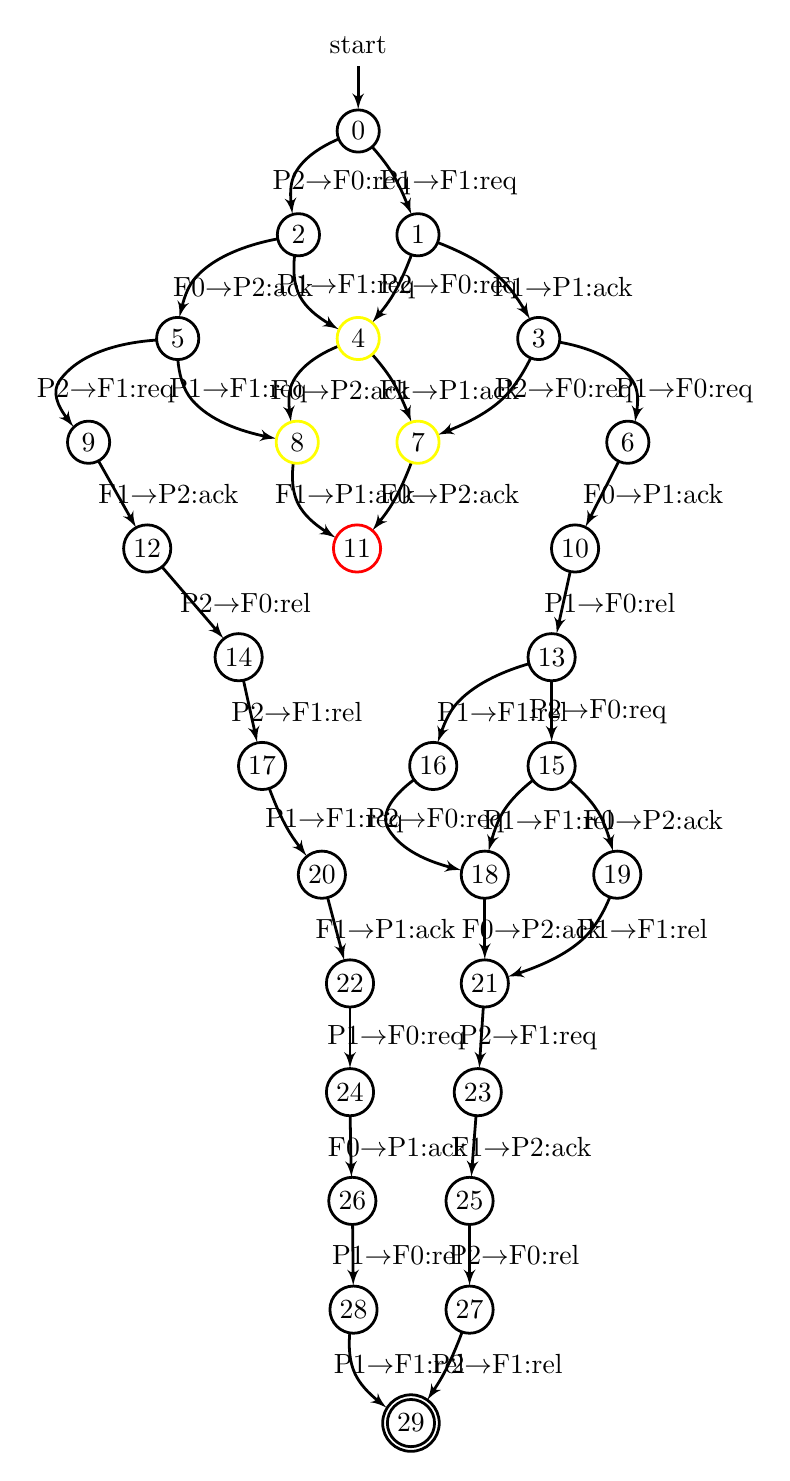
\begin{tikzpicture}[>=latex',line join=bevel,scale=0.422]
  \pgfsetlinewidth{1bp}
%%
\pgfsetcolor{black}
  % Edge: F02F10P10P21 -> F04F10P10P22
  \draw [->] (189.25bp,1034.3bp) .. controls (169.54bp,1030.6bp) and (138.3bp,1021.8bp)  .. (119.97bp,1001.9bp) .. controls (114.12bp,995.5bp) and (110.44bp,987.01bp)  .. (105.68bp,967.53bp);
  \definecolor{strokecol}{rgb}{0.0,0.0,0.0};
  \pgfsetstrokecolor{strokecol}
  \draw (160.09bp,993.61bp) node {F0$\to$P2:ack};
  % Edge: F02F10P10P21 -> F02F11P11P21
  \draw [->] (203.95bp,1020.1bp) .. controls (202.74bp,1009.5bp) and (202.82bp,995.93bp)  .. (208.47bp,985.36bp) .. controls (213.61bp,975.75bp) and (222.68bp,968.2bp)  .. (241.61bp,957.13bp);
  \draw (247.84bp,993.61bp) node {P1$\to$F1:req};
  % Edge: F00F11P11P20 -> F00F13P12P20
  \draw [->] (326.29bp,1031.1bp) .. controls (341.23bp,1025.4bp) and (362.88bp,1015.5bp)  .. (378.22bp,1001.9bp) .. controls (386.47bp,994.5bp) and (393.59bp,984.71bp)  .. (404.75bp,965.88bp);
  \draw (432.79bp,993.61bp) node {F1$\to$P1:ack};
  % Edge: F00F11P11P20 -> F02F11P11P21
  \draw [->] (303.61bp,1020.5bp) .. controls (299.71bp,1010.1bp) and (294.0bp,996.48bp)  .. (287.22bp,985.36bp) .. controls (284.34bp,980.64bp) and (280.86bp,975.88bp)  .. (270.19bp,962.98bp);
  \draw (335.18bp,993.61bp) node {P2$\to$F0:req};
  % Edge: F00F14P16P25 -> F00F10P16P26
  \draw [->] (346.7bp,101.34bp) .. controls (342.73bp,90.805bp) and (337.27bp,77.518bp)  .. (331.22bp,66.262bp) .. controls (328.92bp,61.983bp) and (326.27bp,57.598bp)  .. (317.18bp,43.862bp);
  \draw (376.72bp,74.512bp) node {P2$\to$F1:rel};
  % Edge: F04F12P16P23 -> F04F14P16P24
  \draw [->] (358.73bp,286.17bp) .. controls (357.82bp,274.34bp) and (356.63bp,258.91bp)  .. (354.72bp,234.19bp);
  \draw (397.47bp,260.04bp) node {F1$\to$P2:ack};
  % Edge: F04F13P15P22 -> F04F10P16P22
  \draw [->] (472.84bp,472.57bp) .. controls (468.1bp,461.18bp) and (460.64bp,446.93bp)  .. (450.22bp,437.31bp) .. controls (435.13bp,423.38bp) and (413.97bp,414.07bp)  .. (385.94bp,404.92bp);
  \draw (500.58bp,445.56bp) node {P1$\to$F1:rel};
  % Edge: F03F13P14P26 -> F00F13P15P26
  \draw [->] (253.43bp,193.41bp) .. controls (253.56bp,181.57bp) and (253.73bp,166.15bp)  .. (254.0bp,141.43bp);
  \draw (291.68bp,167.27bp) node {P1$\to$F0:rel};
  % Edge: F00F10P10P26 -> F00F11P11P26
  \draw [->] (182.48bp,565.26bp) .. controls (186.43bp,554.64bp) and (191.99bp,541.23bp)  .. (198.47bp,530.07bp) .. controls (201.07bp,525.59bp) and (204.16bp,521.04bp)  .. (214.22bp,507.83bp);
  \draw (237.84bp,538.32bp) node {P1$\to$F1:req};
  % Edge: F00F10P10P20 -> F02F10P10P21
  \draw [->] (241.27bp,1119.4bp) .. controls (228.61bp,1114.0bp) and (212.22bp,1104.7bp)  .. (204.47bp,1090.4bp) .. controls (200.63bp,1083.3bp) and (199.83bp,1074.8bp)  .. (202.04bp,1055.6bp);
  \draw (243.84bp,1082.1bp) node {P2$\to$F0:req};
  % Edge: F00F10P10P20 -> F00F11P11P20
  \draw [->] (270.19bp,1112.7bp) .. controls (275.83bp,1106.4bp) and (282.37bp,1098.3bp)  .. (287.22bp,1090.4bp) .. controls (291.88bp,1082.7bp) and (296.04bp,1073.9bp)  .. (303.61bp,1055.2bp);
  \draw (335.18bp,1082.1bp) node {P1$\to$F1:req};
  % Edge: F04F10P10P22 -> F04F11P11P22
  \draw [->] (104.36bp,931.24bp) .. controls (105.32bp,920.23bp) and (108.26bp,906.29bp)  .. (116.47bp,896.86bp) .. controls (131.82bp,879.23bp) and (157.16bp,870.42bp)  .. (188.23bp,863.91bp);
  \draw (155.84bp,905.11bp) node {P1$\to$F1:req};
  % Edge: F04F10P10P22 -> F04F12P10P23
  \draw [->] (85.982bp,948.0bp) .. controls (62.433bp,946.43bp) and (22.249bp,939.77bp)  .. (3.468bp,913.36bp) .. controls (-3.2418bp,903.93bp) and (1.3095bp,892.39bp)  .. (15.345bp,873.94bp);
  \draw (42.843bp,905.11bp) node {P2$\to$F1:req};
  % Edge: F00F13P12P26 -> F01F13P13P26
  \draw [->] (251.22bp,378.93bp) .. controls (251.22bp,367.1bp) and (251.22bp,351.67bp)  .. (251.22bp,326.95bp);
  \draw (290.59bp,352.8bp) node {P1$\to$F0:req};
  % Edge: F04F14P10P24 -> F00F14P10P25
  \draw [->] (91.098bp,754.24bp) .. controls (103.29bp,740.05bp) and (121.79bp,718.53bp)  .. (143.32bp,693.48bp);
  \draw (162.08bp,723.85bp) node {P2$\to$F0:rel};
  % Edge: F00F13P15P26 -> F00F10P16P26
  \draw [->] (250.98bp,100.66bp) .. controls (250.07bp,90.03bp) and (250.45bp,76.872bp)  .. (255.47bp,66.262bp) .. controls (259.48bp,57.777bp) and (266.16bp,50.36bp)  .. (282.35bp,37.222bp);
  \draw (293.34bp,74.512bp) node {P1$\to$F1:rel};
  % Edge: F00F13P12P20 -> F01F13P13P20
  \draw [->] (430.17bp,946.17bp) .. controls (449.25bp,942.78bp) and (478.53bp,934.29bp)  .. (492.22bp,913.36bp) .. controls (496.82bp,906.32bp) and (497.52bp,897.53bp)  .. (494.3bp,878.0bp);
  \draw (536.24bp,905.11bp) node {P1$\to$F0:req};
  % Edge: F00F13P12P20 -> F02F13P12P21
  \draw [->] (405.19bp,932.32bp) .. controls (399.68bp,921.23bp) and (391.14bp,906.76bp)  .. (380.22bp,896.86bp) .. controls (367.77bp,885.57bp) and (351.01bp,877.08bp)  .. (326.28bp,867.22bp);
  \draw (433.49bp,905.11bp) node {P2$\to$F0:req};
  % Edge: F02F11P11P21 -> F04F11P11P22
  \draw [->] (241.08bp,942.68bp) .. controls (228.04bp,937.35bp) and (211.02bp,927.98bp)  .. (202.97bp,913.36bp) .. controls (199.02bp,906.19bp) and (198.31bp,897.57bp)  .. (200.87bp,878.16bp);
  \draw (243.09bp,905.11bp) node {F0$\to$P2:ack};
  % Edge: F02F11P11P21 -> F02F13P12P21
  \draw [->] (270.19bp,935.74bp) .. controls (275.83bp,929.37bp) and (282.37bp,921.31bp)  .. (287.22bp,913.36bp) .. controls (291.88bp,905.71bp) and (296.04bp,896.9bp)  .. (303.61bp,878.22bp);
  \draw (335.93bp,905.11bp) node {F1$\to$P1:ack};
  % Edge: F04F14P16P24 -> F00F14P16P25
  \draw [->] (353.22bp,193.41bp) .. controls (353.22bp,181.57bp) and (353.22bp,166.15bp)  .. (353.22bp,141.43bp);
  \draw (391.09bp,167.27bp) node {P2$\to$F0:rel};
  % Edge: F04F11P11P22 -> F04F13P12P22
  \draw [->] (202.78bp,842.71bp) .. controls (201.54bp,832.22bp) and (201.58bp,818.86bp)  .. (206.97bp,808.36bp) .. controls (211.87bp,798.83bp) and (220.47bp,791.12bp)  .. (238.89bp,779.41bp);
  \draw (247.09bp,816.61bp) node {F1$\to$P1:ack};
  % Edge: start_node -> F00F10P10P20
  \draw [->] (258.22bp,1181.5bp) .. controls (258.22bp,1173.9bp) and (258.22bp,1164.7bp)  .. (258.22bp,1144.8bp);
  % Edge: F01F13P13P26 -> F03F13P14P26
  \draw [->] (251.4bp,286.05bp) .. controls (251.51bp,275.86bp) and (251.7bp,263.14bp)  .. (251.97bp,251.79bp) .. controls (252.02bp,249.7bp) and (252.07bp,247.55bp)  .. (252.5bp,233.93bp);
  \draw (292.09bp,260.04bp) node {F0$\to$P1:ack};
  % Edge: F00F11P11P26 -> F00F13P12P26
  \draw [->] (232.19bp,472.14bp) .. controls (235.41bp,459.97bp) and (239.67bp,443.86bp)  .. (246.25bp,418.96bp);
  \draw (281.49bp,445.56bp) node {F1$\to$P1:ack};
  % Edge: F02F10P16P21 -> F04F10P16P22
  \draw [->] (366.22bp,471.69bp) .. controls (366.22bp,459.86bp) and (366.22bp,444.43bp)  .. (366.22bp,419.71bp);
  \draw (406.34bp,445.56bp) node {F0$\to$P2:ack};
  % Edge: F00F10P16P20 -> F02F10P16P21
  \draw [->] (305.57bp,572.79bp) .. controls (291.39bp,562.08bp) and (274.73bp,545.2bp)  .. (284.47bp,530.07bp) .. controls (295.6bp,512.79bp) and (316.96bp,503.46bp)  .. (346.05bp,495.85bp);
  \draw (323.84bp,538.32bp) node {P2$\to$F0:req};
  % Edge: F01F13P13P20 -> F03F13P14P20
  \draw [->] (480.38bp,844.42bp) .. controls (473.96bp,831.77bp) and (464.71bp,813.55bp)  .. (452.04bp,788.61bp);
  \draw (509.87bp,816.61bp) node {F0$\to$P1:ack};
  % Edge: F04F12P10P23 -> F04F14P10P24
  \draw [->] (36.7bp,844.83bp) .. controls (43.899bp,832.06bp) and (54.405bp,813.44bp)  .. (68.669bp,788.16bp);
  \draw (96.337bp,816.61bp) node {F1$\to$P2:ack};
  % Edge: F04F10P16P22 -> F04F12P16P23
  \draw [->] (364.95bp,378.93bp) .. controls (364.16bp,367.1bp) and (363.14bp,351.67bp)  .. (361.51bp,326.95bp);
  \draw (403.13bp,352.8bp) node {P2$\to$F1:req};
  % Edge: F02F13P12P21 -> F04F13P12P22
  \draw [->] (303.57bp,843.53bp) .. controls (299.65bp,833.11bp) and (293.93bp,819.52bp)  .. (287.22bp,808.36bp) .. controls (284.38bp,803.64bp) and (280.99bp,798.86bp)  .. (270.47bp,785.71bp);
  \draw (335.87bp,816.61bp) node {F0$\to$P2:ack};
  % Edge: F03F13P14P20 -> F00F13P15P20
  \draw [->] (439.07bp,750.42bp) .. controls (436.41bp,738.33bp) and (432.89bp,722.36bp)  .. (427.43bp,697.56bp);
  \draw (472.88bp,723.85bp) node {P1$\to$F0:rel};
  % Edge: F00F13P15P20 -> F00F10P16P20
  \draw [->] (403.7bp,671.83bp) .. controls (385.85bp,666.66bp) and (359.82bp,656.67bp)  .. (343.47bp,639.34bp) .. controls (337.21bp,632.7bp) and (332.71bp,624.0bp)  .. (326.03bp,604.75bp);
  \draw (381.34bp,631.09bp) node {P1$\to$F1:rel};
  % Edge: F00F13P15P20 -> F02F13P15P21
  \draw [->] (423.22bp,657.22bp) .. controls (423.22bp,645.39bp) and (423.22bp,629.96bp)  .. (423.22bp,605.24bp);
  \draw (462.59bp,631.09bp) node {P2$\to$F0:req};
  % Edge: F00F14P10P25 -> F00F10P10P26
  \draw [->] (160.36bp,657.66bp) .. controls (163.03bp,645.57bp) and (166.55bp,629.6bp)  .. (172.01bp,604.8bp);
  \draw (205.88bp,631.09bp) node {P2$\to$F1:rel};
  % Edge: F02F13P15P21 -> F04F13P15P22
  \draw [->] (439.12bp,571.79bp) .. controls (447.03bp,565.13bp) and (456.17bp,556.25bp)  .. (462.22bp,546.57bp) .. controls (466.69bp,539.42bp) and (470.07bp,531.0bp)  .. (475.63bp,512.06bp);
  \draw (509.77bp,538.32bp) node {F0$\to$P2:ack};
  % Edge: F02F13P15P21 -> F02F10P16P21
  \draw [->] (406.94bp,572.27bp) .. controls (398.56bp,565.64bp) and (388.8bp,556.61bp)  .. (382.47bp,546.57bp) .. controls (377.99bp,539.47bp) and (374.68bp,531.06bp)  .. (369.41bp,512.11bp);
  \draw (420.34bp,538.32bp) node {P1$\to$F1:rel};
  % Node: F02F10P10P21
\begin{scope}
  \definecolor{strokecol}{rgb}{0.0,0.0,0.0};
  \pgfsetstrokecolor{strokecol}
  \draw (207.22bp,1037.86bp) ellipse (18.0bp and 18.0bp);
  \draw (207.22bp,1037.9bp) node {2};
\end{scope}
  % Node: F04F10P10P22
\begin{scope}
  \definecolor{strokecol}{rgb}{0.0,0.0,0.0};
  \pgfsetstrokecolor{strokecol}
  \draw (104.22bp,949.36bp) ellipse (18.0bp and 18.0bp);
  \draw (104.22bp,949.36bp) node {5};
\end{scope}
  % Node: F02F11P11P21
\begin{scope}
  \definecolor{strokecol}{rgb}{1.0,1.0,0.0};
  \pgfsetstrokecolor{strokecol}
  \draw (258.22bp,949.36bp) ellipse (18.0bp and 18.0bp);
  \definecolor{strokecol}{rgb}{0.0,0.0,0.0};
  \pgfsetstrokecolor{strokecol}
  \draw (258.22bp,949.36bp) node {4};
\end{scope}
  % Node: F00F11P11P20
\begin{scope}
  \definecolor{strokecol}{rgb}{0.0,0.0,0.0};
  \pgfsetstrokecolor{strokecol}
  \draw (309.22bp,1037.86bp) ellipse (18.0bp and 18.0bp);
  \draw (309.22bp,1037.9bp) node {1};
\end{scope}
  % Node: F00F13P12P20
\begin{scope}
  \definecolor{strokecol}{rgb}{0.0,0.0,0.0};
  \pgfsetstrokecolor{strokecol}
  \draw (412.22bp,949.36bp) ellipse (18.0bp and 18.0bp);
  \draw (412.22bp,949.36bp) node {3};
\end{scope}
  % Node: F00F14P16P25
\begin{scope}
  \definecolor{strokecol}{rgb}{0.0,0.0,0.0};
  \pgfsetstrokecolor{strokecol}
  \draw (353.22bp,120.89bp) ellipse (20.13bp and 20.13bp);
  \draw (353.22bp,120.89bp) node {27};
\end{scope}
  % Node: F00F10P16P26
\begin{scope}
  \definecolor{strokecol}{rgb}{0.0,0.0,0.0};
  \pgfsetstrokecolor{strokecol}
  \draw (303.22bp,24.13bp) ellipse (20.13bp and 20.13bp);
  \draw (303.22bp,24.13bp) ellipse (24.13bp and 24.13bp);
  \draw (303.22bp,24.131bp) node {29};
\end{scope}
  % Node: F04F12P16P23
\begin{scope}
  \definecolor{strokecol}{rgb}{0.0,0.0,0.0};
  \pgfsetstrokecolor{strokecol}
  \draw (360.22bp,306.42bp) ellipse (20.13bp and 20.13bp);
  \draw (360.22bp,306.42bp) node {23};
\end{scope}
  % Node: F04F14P16P24
\begin{scope}
  \definecolor{strokecol}{rgb}{0.0,0.0,0.0};
  \pgfsetstrokecolor{strokecol}
  \draw (353.22bp,213.66bp) ellipse (20.13bp and 20.13bp);
  \draw (353.22bp,213.66bp) node {25};
\end{scope}
  % Node: F04F13P15P22
\begin{scope}
  \definecolor{strokecol}{rgb}{0.0,0.0,0.0};
  \pgfsetstrokecolor{strokecol}
  \draw (479.22bp,491.94bp) ellipse (20.13bp and 20.13bp);
  \draw (479.22bp,491.94bp) node {19};
\end{scope}
  % Node: F04F10P16P22
\begin{scope}
  \definecolor{strokecol}{rgb}{0.0,0.0,0.0};
  \pgfsetstrokecolor{strokecol}
  \draw (366.22bp,399.18bp) ellipse (20.13bp and 20.13bp);
  \draw (366.22bp,399.18bp) node {21};
\end{scope}
  % Node: F03F13P14P26
\begin{scope}
  \definecolor{strokecol}{rgb}{0.0,0.0,0.0};
  \pgfsetstrokecolor{strokecol}
  \draw (253.22bp,213.66bp) ellipse (20.13bp and 20.13bp);
  \draw (253.22bp,213.66bp) node {26};
\end{scope}
  % Node: F00F13P15P26
\begin{scope}
  \definecolor{strokecol}{rgb}{0.0,0.0,0.0};
  \pgfsetstrokecolor{strokecol}
  \draw (254.22bp,120.89bp) ellipse (20.13bp and 20.13bp);
  \draw (254.22bp,120.89bp) node {28};
\end{scope}
  % Node: F00F10P10P26
\begin{scope}
  \definecolor{strokecol}{rgb}{0.0,0.0,0.0};
  \pgfsetstrokecolor{strokecol}
  \draw (176.22bp,584.7bp) ellipse (20.13bp and 20.13bp);
  \draw (176.22bp,584.7bp) node {17};
\end{scope}
  % Node: F00F11P11P26
\begin{scope}
  \definecolor{strokecol}{rgb}{0.0,0.0,0.0};
  \pgfsetstrokecolor{strokecol}
  \draw (227.22bp,491.94bp) ellipse (20.13bp and 20.13bp);
  \draw (227.22bp,491.94bp) node {20};
\end{scope}
  % Node: F00F10P10P20
\begin{scope}
  \definecolor{strokecol}{rgb}{0.0,0.0,0.0};
  \pgfsetstrokecolor{strokecol}
  \draw (258.22bp,1126.36bp) ellipse (18.0bp and 18.0bp);
  \draw (258.22bp,1126.4bp) node {0};
\end{scope}
  % Node: F04F11P11P22
\begin{scope}
  \definecolor{strokecol}{rgb}{1.0,1.0,0.0};
  \pgfsetstrokecolor{strokecol}
  \draw (206.22bp,860.86bp) ellipse (18.0bp and 18.0bp);
  \definecolor{strokecol}{rgb}{0.0,0.0,0.0};
  \pgfsetstrokecolor{strokecol}
  \draw (206.22bp,860.86bp) node {8};
\end{scope}
  % Node: F04F12P10P23
\begin{scope}
  \definecolor{strokecol}{rgb}{0.0,0.0,0.0};
  \pgfsetstrokecolor{strokecol}
  \draw (28.22bp,860.86bp) ellipse (18.0bp and 18.0bp);
  \draw (28.218bp,860.86bp) node {9};
\end{scope}
  % Node: F00F13P12P26
\begin{scope}
  \definecolor{strokecol}{rgb}{0.0,0.0,0.0};
  \pgfsetstrokecolor{strokecol}
  \draw (251.22bp,399.18bp) ellipse (20.13bp and 20.13bp);
  \draw (251.22bp,399.18bp) node {22};
\end{scope}
  % Node: F01F13P13P26
\begin{scope}
  \definecolor{strokecol}{rgb}{0.0,0.0,0.0};
  \pgfsetstrokecolor{strokecol}
  \draw (251.22bp,306.42bp) ellipse (20.13bp and 20.13bp);
  \draw (251.22bp,306.42bp) node {24};
\end{scope}
  % Node: F04F14P10P24
\begin{scope}
  \definecolor{strokecol}{rgb}{0.0,0.0,0.0};
  \pgfsetstrokecolor{strokecol}
  \draw (78.22bp,770.23bp) ellipse (20.13bp and 20.13bp);
  \draw (78.218bp,770.23bp) node {12};
\end{scope}
  % Node: F00F14P10P25
\begin{scope}
  \definecolor{strokecol}{rgb}{0.0,0.0,0.0};
  \pgfsetstrokecolor{strokecol}
  \draw (156.22bp,677.47bp) ellipse (20.13bp and 20.13bp);
  \draw (156.22bp,677.47bp) node {14};
\end{scope}
  % Node: F01F13P13P20
\begin{scope}
  \definecolor{strokecol}{rgb}{0.0,0.0,0.0};
  \pgfsetstrokecolor{strokecol}
  \draw (488.22bp,860.86bp) ellipse (18.0bp and 18.0bp);
  \draw (488.22bp,860.86bp) node {6};
\end{scope}
  % Node: F02F13P12P21
\begin{scope}
  \definecolor{strokecol}{rgb}{1.0,1.0,0.0};
  \pgfsetstrokecolor{strokecol}
  \draw (309.22bp,860.86bp) ellipse (18.0bp and 18.0bp);
  \definecolor{strokecol}{rgb}{0.0,0.0,0.0};
  \pgfsetstrokecolor{strokecol}
  \draw (309.22bp,860.86bp) node {7};
\end{scope}
  % Node: F04F13P12P22
\begin{scope}
  \definecolor{strokecol}{rgb}{1.0,0.0,0.0};
  \pgfsetstrokecolor{strokecol}
  \draw (257.22bp,770.23bp) ellipse (20.13bp and 20.13bp);
  \definecolor{strokecol}{rgb}{0.0,0.0,0.0};
  \pgfsetstrokecolor{strokecol}
  \draw (257.22bp,770.23bp) node {11};
\end{scope}
  % Node: start_node
\begin{scope}
  \definecolor{strokecol}{rgb}{0.0,0.0,0.0};
  \pgfsetstrokecolor{strokecol}
  \draw (258.22bp,1199.4bp) node {start};
\end{scope}
  % Node: F02F10P16P21
\begin{scope}
  \definecolor{strokecol}{rgb}{0.0,0.0,0.0};
  \pgfsetstrokecolor{strokecol}
  \draw (366.22bp,491.94bp) ellipse (20.13bp and 20.13bp);
  \draw (366.22bp,491.94bp) node {18};
\end{scope}
  % Node: F00F10P16P20
\begin{scope}
  \definecolor{strokecol}{rgb}{0.0,0.0,0.0};
  \pgfsetstrokecolor{strokecol}
  \draw (322.22bp,584.7bp) ellipse (20.13bp and 20.13bp);
  \draw (322.22bp,584.7bp) node {16};
\end{scope}
  % Node: F03F13P14P20
\begin{scope}
  \definecolor{strokecol}{rgb}{0.0,0.0,0.0};
  \pgfsetstrokecolor{strokecol}
  \draw (443.22bp,770.23bp) ellipse (20.13bp and 20.13bp);
  \draw (443.22bp,770.23bp) node {10};
\end{scope}
  % Node: F00F13P15P20
\begin{scope}
  \definecolor{strokecol}{rgb}{0.0,0.0,0.0};
  \pgfsetstrokecolor{strokecol}
  \draw (423.22bp,677.47bp) ellipse (20.13bp and 20.13bp);
  \draw (423.22bp,677.47bp) node {13};
\end{scope}
  % Node: F02F13P15P21
\begin{scope}
  \definecolor{strokecol}{rgb}{0.0,0.0,0.0};
  \pgfsetstrokecolor{strokecol}
  \draw (423.22bp,584.7bp) ellipse (20.13bp and 20.13bp);
  \draw (423.22bp,584.7bp) node {15};
\end{scope}
%
\end{tikzpicture}

    \caption{Synchronous Product of the Example~\ref{exm:philo}.}
    \label{fig:philo-sync}
\end{figure}

\end{example}

\begin{example}\label{exm:loop}
Now consider two processes $A$ and $B$ that exchange data. At some
point, each makes a nondeterministic choice: one branch continues
sending messages indefinitely, while the other leads to termination.
Once the choice to continue is taken, however, there is no way to
return to the terminating branch. As a result, the system may remain
stuck in an infinite loop, never reaching a final state. Although both
processes remain active, the system is effectively deadlocked.

\begin{lstlisting}[language={},caption={Output of Example~\ref{exm:loop}.},
    label={lst:loop}]
This system is RSC.
The system has the progress property.
There are some deadlock states:
Deadlock: Id=17 Configuration={{ A:1; B:4 }}
Deadlock: Id=15 Configuration={{ A:3; B:3 }}
\end{lstlisting}

The behavior of this system is shown in Figure~\ref{fig:loop}. 
Executing the tool produces the output in
Listing~\ref{lst:loop} and the synchronous system in
Figure~\ref{fig:loop-sync}. In the
generated figure, yellow states highlight the deadlocked executions,
while the terminal output provides the configuration of each detected
deadlock.


\begin{figure}[!ht]
    \centering
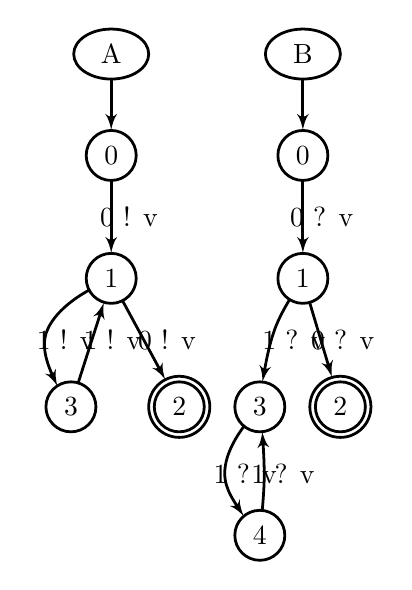
\begin{tikzpicture}[>=latex',line join=bevel,scale=0.5]
  \pgfsetlinewidth{1bp}
%%
\pgfsetcolor{black}
  % Edge: B3 -> B4
  \draw [->] (144.22bp,96.57bp) .. controls (135.94bp,85.51bp) and (126.9bp,69.041bp)  .. (131.56bp,54.0bp) .. controls (132.92bp,49.613bp) and (135.04bp,45.286bp)  .. (143.89bp,31.954bp);
  \definecolor{strokecol}{rgb}{0.0,0.0,0.0};
  \pgfsetstrokecolor{strokecol}
  \draw (145.06bp,62.25bp) node {1 ? v};
  % Edge: B4 -> B3
  \draw [->] (157.32bp,36.071bp) .. controls (157.82bp,41.766bp) and (158.31bp,48.151bp)  .. (158.56bp,54.0bp) .. controls (158.94bp,62.881bp) and (158.66bp,72.558bp)  .. (157.33bp,92.502bp);
  \draw (172.23bp,62.25bp) node {1 ? v};
  % Edge: Bdummy -> B0
  \draw [->] (186.56bp,346.67bp) .. controls (186.56bp,339.06bp) and (186.56bp,329.85bp)  .. (186.56bp,309.95bp);
  % Edge: A3 -> A1
  \draw [->] (24.844bp,127.99bp) .. controls (29.004bp,140.98bp) and (34.892bp,159.35bp)  .. (43.239bp,185.4bp);
  \draw (49.406bp,158.75bp) node {1 ! v};
  % Edge: B0 -> B1
  \draw [->] (186.56bp,273.41bp) .. controls (186.56bp,261.76bp) and (186.56bp,246.05bp)  .. (186.56bp,221.35bp);
  \draw (200.06bp,247.25bp) node {0 ? v};
  % Edge: A1 -> A2
  \draw [->] (56.87bp,186.65bp) .. controls (63.703bp,174.03bp) and (73.577bp,155.79bp)  .. (87.333bp,130.39bp);
  \draw (88.742bp,158.75bp) node {0 ! v};
  % Edge: A1 -> A3
  \draw [->] (32.341bp,194.41bp) .. controls (21.881bp,188.55bp) and (9.1337bp,179.34bp)  .. (3.0583bp,167.0bp) .. controls (-1.7681bp,157.2bp) and (0.47788bp,145.72bp)  .. (9.7171bp,125.67bp);
  \draw (15.808bp,158.75bp) node {1 ! v};
  % Edge: A0 -> A1
  \draw [->] (48.558bp,273.41bp) .. controls (48.558bp,261.76bp) and (48.558bp,246.05bp)  .. (48.558bp,221.35bp);
  \draw (61.308bp,247.25bp) node {0 ! v};
  % Edge: B1 -> B3
  \draw [->] (176.88bp,187.53bp) .. controls (173.18bp,181.42bp) and (169.2bp,174.08bp)  .. (166.56bp,167.0bp) .. controls (163.37bp,158.46bp) and (161.05bp,148.82bp)  .. (157.5bp,128.65bp);
  \draw (180.06bp,158.75bp) node {1 ? v};
  % Edge: B1 -> B2
  \draw [->] (191.51bp,185.4bp) .. controls (195.04bp,173.56bp) and (199.9bp,157.28bp)  .. (207.41bp,132.12bp);
  \draw (215.17bp,158.75bp) node {0 ? v};
  % Edge: Adummy -> A0
  \draw [->] (48.558bp,346.67bp) .. controls (48.558bp,339.06bp) and (48.558bp,329.85bp)  .. (48.558bp,309.95bp);
  % Node: A2
\begin{scope}
  \definecolor{strokecol}{rgb}{0.0,0.0,0.0};
  \pgfsetstrokecolor{strokecol}
  \draw (97.56bp,110.5bp) ellipse (18.0bp and 18.0bp);
  \draw (97.56bp,110.5bp) ellipse (22.0bp and 22.0bp);
  \draw (97.558bp,110.5bp) node {2};
\end{scope}
  % Node: B3
\begin{scope}
  \definecolor{strokecol}{rgb}{0.0,0.0,0.0};
  \pgfsetstrokecolor{strokecol}
  \draw (155.56bp,110.5bp) ellipse (18.0bp and 18.0bp);
  \draw (155.56bp,110.5bp) node {3};
\end{scope}
  % Node: B4
\begin{scope}
  \definecolor{strokecol}{rgb}{0.0,0.0,0.0};
  \pgfsetstrokecolor{strokecol}
  \draw (155.56bp,18.0bp) ellipse (18.0bp and 18.0bp);
  \draw (155.56bp,18.0bp) node {4};
\end{scope}
  % Node: Bdummy
\begin{scope}
  \definecolor{strokecol}{rgb}{0.0,0.0,0.0};
  \pgfsetstrokecolor{strokecol}
  \draw (186.56bp,364.5bp) ellipse (27.0bp and 18.0bp);
  \draw (186.56bp,364.5bp) node {B};
\end{scope}
  % Node: B0
\begin{scope}
  \definecolor{strokecol}{rgb}{0.0,0.0,0.0};
  \pgfsetstrokecolor{strokecol}
  \draw (186.56bp,291.5bp) ellipse (18.0bp and 18.0bp);
  \draw (186.56bp,291.5bp) node {0};
\end{scope}
  % Node: A3
\begin{scope}
  \definecolor{strokecol}{rgb}{0.0,0.0,0.0};
  \pgfsetstrokecolor{strokecol}
  \draw (19.56bp,110.5bp) ellipse (18.0bp and 18.0bp);
  \draw (19.558bp,110.5bp) node {3};
\end{scope}
  % Node: A1
\begin{scope}
  \definecolor{strokecol}{rgb}{0.0,0.0,0.0};
  \pgfsetstrokecolor{strokecol}
  \draw (48.56bp,203.0bp) ellipse (18.0bp and 18.0bp);
  \draw (48.558bp,203.0bp) node {1};
\end{scope}
  % Node: B1
\begin{scope}
  \definecolor{strokecol}{rgb}{0.0,0.0,0.0};
  \pgfsetstrokecolor{strokecol}
  \draw (186.56bp,203.0bp) ellipse (18.0bp and 18.0bp);
  \draw (186.56bp,203.0bp) node {1};
\end{scope}
  % Node: B2
\begin{scope}
  \definecolor{strokecol}{rgb}{0.0,0.0,0.0};
  \pgfsetstrokecolor{strokecol}
  \draw (213.56bp,110.5bp) ellipse (18.0bp and 18.0bp);
  \draw (213.56bp,110.5bp) ellipse (22.0bp and 22.0bp);
  \draw (213.56bp,110.5bp) node {2};
\end{scope}
  % Node: A0
\begin{scope}
  \definecolor{strokecol}{rgb}{0.0,0.0,0.0};
  \pgfsetstrokecolor{strokecol}
  \draw (48.56bp,291.5bp) ellipse (18.0bp and 18.0bp);
  \draw (48.558bp,291.5bp) node {0};
\end{scope}
  % Node: Adummy
\begin{scope}
  \definecolor{strokecol}{rgb}{0.0,0.0,0.0};
  \pgfsetstrokecolor{strokecol}
  \draw (48.56bp,364.5bp) ellipse (27.0bp and 18.0bp);
  \draw (48.558bp,364.5bp) node {A};
\end{scope}
%
\end{tikzpicture}
    \caption{SCM automata representation of the Example~\ref{exm:loop}.}
    \label{fig:loop}
\end{figure}


\begin{figure}[!ht]
    \centering

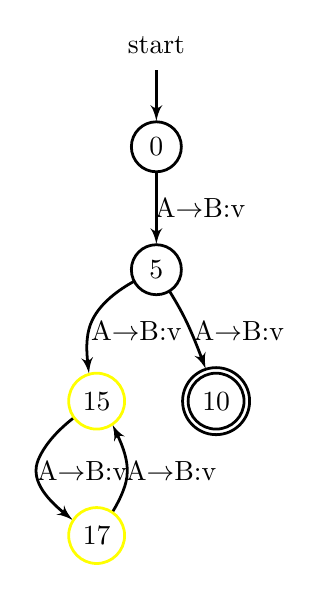
\begin{tikzpicture}[>=latex',line join=bevel,scale=0.5]
  \pgfsetlinewidth{1bp}
%%
\pgfsetcolor{black}
  % Edge: A3B3 -> A1B4
  \draw [->] (27.548bp,105.03bp) .. controls (18.113bp,97.729bp) and (7.1099bp,87.181bp)  .. (1.8895bp,74.762bp) .. controls (-3.8439bp,61.122bp) and (6.0577bp,48.005bp)  .. (26.676bp,31.31bp);
  \definecolor{strokecol}{rgb}{0.0,0.0,0.0};
  \pgfsetstrokecolor{strokecol}
  \draw (33.39bp,66.512bp) node {A$\to$B:v};
  % Edge: A0B0 -> A1B1
  \draw [->] (86.89bp,281.93bp) .. controls (86.89bp,270.28bp) and (86.89bp,254.57bp)  .. (86.89bp,229.87bp);
  \draw (118.39bp,255.77bp) node {A$\to$B:v};
  % Edge: start_node -> A0B0
  \draw [->] (86.89bp,355.2bp) .. controls (86.89bp,347.59bp) and (86.89bp,338.37bp)  .. (86.89bp,318.47bp);
  % Edge: A1B1 -> A3B3
  \draw [->] (70.499bp,202.98bp) .. controls (59.926bp,197.13bp) and (47.04bp,187.93bp)  .. (40.89bp,175.52bp) .. controls (36.728bp,167.13bp) and (36.008bp,157.18bp)  .. (38.379bp,136.75bp);
  \draw (72.39bp,167.27bp) node {A$\to$B:v};
  % Edge: A1B1 -> A2B2
  \draw [->] (96.475bp,195.86bp) .. controls (100.28bp,189.71bp) and (104.54bp,182.41bp)  .. (107.89bp,175.52bp) .. controls (111.69bp,167.71bp) and (115.29bp,159.06bp)  .. (122.42bp,140.17bp);
  \draw (146.28bp,167.27bp) node {A$\to$B:v};
  % Edge: A1B4 -> A3B3
  \draw [->] (55.235bp,36.979bp) .. controls (59.096bp,43.289bp) and (62.929bp,50.814bp)  .. (64.89bp,58.262bp) .. controls (67.676bp,68.85bp) and (64.837bp,80.229bp)  .. (55.255bp,99.999bp);
  \draw (97.489bp,66.512bp) node {A$\to$B:v};
  % Node: A3B3
\begin{scope}
  \definecolor{strokecol}{rgb}{1.0,1.0,0.0};
  \pgfsetstrokecolor{strokecol}
  \draw (43.89bp,116.89bp) ellipse (20.13bp and 20.13bp);
  \definecolor{strokecol}{rgb}{0.0,0.0,0.0};
  \pgfsetstrokecolor{strokecol}
  \draw (43.89bp,116.89bp) node {15};
\end{scope}
  % Node: A1B4
\begin{scope}
  \definecolor{strokecol}{rgb}{1.0,1.0,0.0};
  \pgfsetstrokecolor{strokecol}
  \draw (43.89bp,20.13bp) ellipse (20.13bp and 20.13bp);
  \definecolor{strokecol}{rgb}{0.0,0.0,0.0};
  \pgfsetstrokecolor{strokecol}
  \draw (43.89bp,20.131bp) node {17};
\end{scope}
  % Node: A2B2
\begin{scope}
  \definecolor{strokecol}{rgb}{0.0,0.0,0.0};
  \pgfsetstrokecolor{strokecol}
  \draw (129.89bp,116.89bp) ellipse (20.13bp and 20.13bp);
  \draw (129.89bp,116.89bp) ellipse (24.13bp and 24.13bp);
  \draw (129.89bp,116.89bp) node {10};
\end{scope}
  % Node: A0B0
\begin{scope}
  \definecolor{strokecol}{rgb}{0.0,0.0,0.0};
  \pgfsetstrokecolor{strokecol}
  \draw (86.89bp,300.02bp) ellipse (18.0bp and 18.0bp);
  \draw (86.89bp,300.02bp) node {0};
\end{scope}
  % Node: A1B1
\begin{scope}
  \definecolor{strokecol}{rgb}{0.0,0.0,0.0};
  \pgfsetstrokecolor{strokecol}
  \draw (86.89bp,211.52bp) ellipse (18.0bp and 18.0bp);
  \draw (86.89bp,211.52bp) node {5};
\end{scope}
  % Node: start_node
\begin{scope}
  \definecolor{strokecol}{rgb}{0.0,0.0,0.0};
  \pgfsetstrokecolor{strokecol}
  \draw (86.89bp,373.02bp) node {start};
\end{scope}
%
\end{tikzpicture}

    \caption{Synchronous Product of the Loop example}
    \label{fig:loop-sync}
\end{figure}


\end{example}



\chapter{Related work}\label{sec:rel}
This thesis is centred around the study of the \emph{implementability 
problem} for \emph{global types} and MSC-based formal models.  
In this chapter, I review related works addressing this problem, 
both within the same formal framework and in comparable models.  

In particular, this thesis forms part of a broader line of research 
originating from~\cite{di2023partial} and later expanded in 
\cite{di2025realisability}, which aims to develop a general framework 
for communication models. I first present and discuss the results of 
these works, positioning my own contributions in relation to them.  

Subsequently, I analyse recent results by 
Stutz~et~al.~\cite{stutz2024implementability}, who extensively study 
the implementability problem, while also tracing the line of research 
back to early contributions such as Alur~et~al.~\cite{alur2000inference} 
and Lohrey~et~al.~\cite{lohrey2003realizability}.  

Finally, I briefly review related approaches in comparable formal 
models, such as Multiparty Session Types (MPST) and Choreography 
Automata~\cite{barbanera2020choreography}, highlighting similarities 
and differences with respect to the problem addressed in this thesis.

\section{Hierarchy of communication model's semantics}\label{sec:hier}
We defined early some communication semantics of out interest.
Furthermore, \cite{di2023partial} show some other interesting 
semantics. It also introduces a hierarchy of communication
semantics, illustrated in Figure~\ref{fig:coms}. The main objective of
this work was to establish a hierarchy that preserves monotonic
properties: if a property holds for a given communication semantic, it
should also hold for all semantics contained within it. However, it was
shown that this monotonicity only applies to specific properties, such
as \emph{weak-$k$-synchronizability}. In contrast, it does not generally
extend to the implementability problem.

% TODO: rsc =/= sync (messaggi orfani)

\begin{figure}[!ht]
\centering
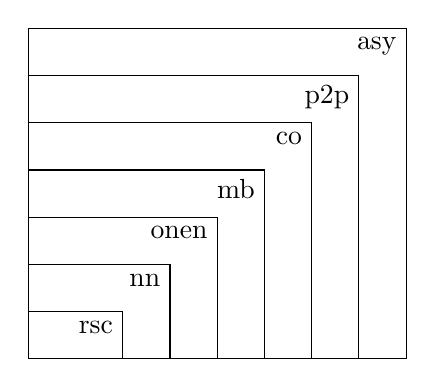
\begin{tikzpicture}[scale=0.6]
  % list of labels in order (from smallest to largest)
%   \def\labels{{rsc,nn,onen,mb,co,p2p,asy}}
  % loop to draw nested squares
  \foreach [count=\i] \lab in {rsc,nn,onen,mb,co,p2p,asy} {
    \draw (0,0) rectangle (\i+1,\i);
    \node[anchor=north east] at (\i+1,\i) {\lab};
  }
\end{tikzpicture}
\caption{Hierarchy of communication model semantics.}
\label{fig:coms}
\end{figure}

% A p2p-MSC is an MSC $M = (E,\to, \lhd, \lambda)$ where, for any two send events $s$ 
% and $s'$ such that $\lambda(s) \in \text{send}(p, q, \_), \lambda(s') in \text{send}(p, q, \_)$, 
% and $s \to^+ s'$, one of the following holds:
% - either $s, s' \in \text{matched}(M)$ with $s \lhd r$ and $s' \lhd r'$ and 
% $r \to^+ r'$,
% - or $s' \in \text{unmatched}(M)$.
% Note that we cannot have two messages $m 1$ and $m 2$, both sent by $p$ to $q$, 
% in that order, such that $m 1$ is unmatched and $m 2$ is matched; unmatched 
% message $m 1$ excludes the reception of any later message.

\paragraph{Peer-to-peer}
In the peer-to-peer communication model $\ppmodel$, every pair of 
processes $(p,q)$ is connected by a dedicated FIFO channel.  
Messages sent by $p$ to $q$ are delivered in the same order in which 
they were issued: if $p$ first sends $m_1$ and then $m_2$, the channel 
guarantees that $m_2$ cannot overtake $m_1$. Concretely:
\begin{itemize}
    \item if $m_1$ is never received, then $m_2$ cannot be received either;
    \item if both are received, then $m_1$ is delivered before $m_2$.
\end{itemize}

\paragraph{Causally ordered}
In the causally ordered (\verb|co|) communication model, messages are delivered 
to a process in accordance with the causal dependencies of their emissions. 
In other words, if there are two messages $m_1$ and $m_2$ with the same recipient, 
such that there exists a causal path from $m_1$ to $m_2$, then $m_1$ must be received 
before $m_2$. This notion of causal ordering was first introduced by Lamport under the 
name ``happened-before'' relation. In Figure~\ref{fig:p2p}, this 
causality is violated: $m_1$ should be received before $m_3$. Causal delivery 
is commonly implemented using Lamport's logical clock algorithm \cite{lamport2019time}.

% An MSC $M = (E, \to, \lhd, \lambda)$ is causally ordered if, for any two send $s$ and 
% $s'$, such that $\lambda(s) \in \text{send}(\_, q, \_), \lambda(s') \in \text{send}(\_, q, \_)$, and 
% $s \leq_{\text{hb}} s'$:
% - either $s, s' \in \text{matched}(M)$ and $r \to^* r'$, with $r$ and $r'$ receive 
% events such that $s \lhd r$ and $s' \lhd r'$.
% - or $s' \in \text{unmatched}(M)$.

% Note that in a \verb|co|-MSC we cannot have two send events $s$ and $s'$ addressed 
% to the same process, such that $s$ is unmatched, $s'$ is matched, and 
% $s \leq_{\text{hb}} s'$.

\paragraph{Mailbox}
In this model, any two messages sent to the same process, regardless of the sender, 
must be received in the same order as they are sent. If a process receives $m_1$ 
before $m_2$, then $m_1$ must have been sent before $m_2$. \verb|mb| coordinates all 
the senders of a single receiver. This model is also called FIFO $n-1$.
In Figure~\ref{fig:mailbox}, an example for this communication model is shown.

\begin{figure}[!ht]
	\centering
	\begin{msc}[draw frame=none, draw head=none, msc keyword=, 
				head height=0px, label distance=0.5ex, 
				foot height=0px, foot distance=0px]{}
		\declinst{p}{p}{}
		\declinst{q}{q}{}
		\declinst{r}{r}{}
		\declinst{s}{s}{}

		\mess[pos=0.1]{$m_4$}{p}{s}[4]
		\nextlevel
		\mess[pos=0.8]{$m_1$}{p}{q}
		\nextlevel
		\mess[pos=0.2]{$m_2$}{r}{q}
		\nextlevel
		\mess[pos=0.8]{$m_3$}{r}{s}
	\end{msc}
	\caption{An example of mailbox semantic.}
	\label{fig:mailbox}
\end{figure}

% An MSC $M = (E, \to, \lhd, \lambda)$ is a \verb|mb|-MSC if it has a linearization 
% $\rightsquigarrow$ where, for any two send events $s$ and $s'$, such 
% that $\lambda (s) \in \text{send}(\_,q,\_), \lambda (s') \in \text{send}(\_,q,\_)$, and 
% $s \rightsquigarrow s'$
% - either $s,s' \in \text{matched}(M)$ and $r \rightsquigarrow r'$, where 
% $s \lhd r$ and $s' \lhd r'$,
% - or $s' \in \text{unmatched}(M)$.

%% TODO: Esistono nella pratica? forse si possono togliere?

\paragraph{FIFO 1-n}
This model (\verb|onen|) is the dual of \verb|mb|, it coordinates a sender with all the 
receivers. Any two messages sent by a process must be received in the same 
order as they are sent. These two messages might be received by different 
processes and the two receive events might be concurrent.

% An MSC $M = (E, \to, \lhd, \lambda)$ is a \verb|onen|-MSC if it has a linearization 
% $\rightsquigarrow$ where, for any two send events $s$ and $s'$, such 
% that $\lambda (s) \in \text{send}(p,\_,\_), \lambda (s') \in \text{send}(p,\_,\_)$ and 
% $s \to^+ s'$ (which implies $s \rightsquigarrow s'$)
% - either $s,s' \in \text{matched}(M)$ and $r \rightsquigarrow r'$, with 
% $r$ and $r'$ receive events such that $s \lhd r$ and $s' \lhd r'$,
% - or $s' \in \text{unmatched}(M)$.

\paragraph{FIFO n-n}
In this model (\verb|nn|), messages are globally ordered and delivered according to 
their emission order. Any two messages must be received in the same order 
as they are sent. These two messages might be sent or receives by any process 
and the two send or receive events might be concurrent. The FIFO \verb|n-n| 
coordinates all the senders with all the receivers.

% An MSC $M = (E, \to, \lhd, \lambda)$ is a \verb|nn|-MSC if it has a linearization 
% $\rightsquigarrow$ where, for any two send events $s$ and $s'$, such 
% that $s \rightsquigarrow s'$
% - either $s, s' \in \text{matched}(M)$ and $r \rightsquigarrow r'$, with $r$ 
% and $r'$ receive events such that $s \lhd r$ and $s' \lhd r'$,
% - or $s' \in \text{unmatched}(M)$.
\paragraph{RSC}
Figure~\ref{fig:coms} shows \verb|rsc| as the last block of the hierarchy.
\verb|rsc| stands for \emph{Realisable in Synchronous Communication}, therefore, 
is comparable to our definition of $\synchmodel$ model, but there are 
some differences. For example, it does not accept \emph{orphan messages}, 
which are instead accepted for the defintion of this thesis.

\section{Realisability for MSCs}

For finite sets of MSCs, weakly realisability as defined in 
\cite{alur2005realizability} is \verb|coNP|-complete and safe 
realisability is shown to be decidable in \verb|P|-time~\cite{alur2005realizability}.
The problem was subsequently studied for infinite MSC languages, defined 
as MSC-Graphs (MSGs). For bounded MSGs, safe realisability 
remains decidable, but weak realisability 
is undecidable~\cite{alur2005realizability}. Extensions of these results to non-FIFO 
semantics were investigated in~\cite{morin2002recognizable}, corresponding 
to bag semantics under peer-to-peer communication. 
Later, Lohrey proved that in the general case, safe realisability 
is undecidable~\cite{lohrey2003realizability}, though it is decidable (and 
\verb|EXPSPACE|-complete) for MSGs. %for globally cooperative MSGs.
Most positive results assume bounded channels, but \cite{bollig2025high} introduces 
a new class of HMSCs that allows unbounded channels while maintaining implementability.
A summary of the main complexity results is given in Table~\ref{tab:realisability}.

\begin{table}[!ht]
	\centering
	\begin{tabular}{|l|c|c|c|}
		\hline
		& \textbf{Finite set} & \textbf{Bounded graphs} & \textbf{Unbounded} \\
		\hline
		\textbf{Weak} & \verb|coNp|-complete & undecidable & undecidable \\
		\hline
		\textbf{Safe} & P-time & \verb|EXPSPACE|-complete & undecidable \\
		\hline
	\end{tabular}
	\caption{Summary of results on realisability.}
	\label{tab:realisability}
\end{table}

\section{Realisability for MPST}

Recent work has focused on strengthening the connection between MPST 
and automata-theoretic formalisms. Stutz and Zufferey 
showed that implementability is decidable by encoding global types 
into HMSCs that are globally cooperative~\cite{stutz2022comparing,stutz2023asynchronous}. 
Building on this, Li et al.~\cite{li2023complete} proposed a complete 
projection function for MPST, guaranteeing that every implementable 
global type admits a correct distributed implementation.

Stutz’s thesis~\cite{stutz2024implementability} connects MPST to 
High-level MSCs (HMSCs), introducing a generalized projection operator 
for sender-driven choice where a sender may branch towards different 
receivers. This captures patterns beyond classical MPST projection.  
He also proves that while syntactic projection is incomplete, 
an automata-theoretic encoding into HMSCs yields decidability for 
sender-driven choice, with implementability shown to be in 
\verb|PSPACE|-the first precise complexity bound for this fragment.

\section{Choreographies}
Choreographies \cite{montesi2014choreographic} are another formalism to describe  
distributed communication protocols. Unlike MSCs or MPST, which focus either on 
trace-based semantics or type systems, choreographies emphasize the 
global specification of interactions as a high-level description of the 
intended message exchanges. Similarly to MPST, their goal is to ensure that
a distributed  implementation can be derived in which each participant 
follows a local behaviour consistent with the global description, called
respectively \emph{local} and \emph{global-view}. This setting naturally 
connects to the realisability problem, since the key question is whether 
a choreography can be faithfully implemented by a system of local 
processes. In choreographies, the local-view is called \textbf{End-Point Projection} (EPP),
and it is derived throughout a projection operation from the global-view.
The \emph{knowledge of choice} problem is similar to the implementability one,
and explored also in choreographies,
but it was first introduced by Castagna et al.~\cite{castagna2012global}.
% https://www.fabriziomontesi.com/bliki/KnowledgeOfChoice#CHY12
% TODO: Continuare menzionando che i chor automata sono simili alla nostra 
% definizione di global type

\section{Other works}
%citare il paper di Emilio su pomsets
Stutz et al.~\cite{stutz2025automata} proposed \emph{Protocol State Machines} 
(PSMs), an automata-based formalism subsuming both MPST and HMSCs. 
PSMs show that many syntactic restrictions of global types are not 
true expressivity limits. Yet, the implementability problem for PSMs 
with unrestricted mixed choice remains undecidable, resolving the 
open question that mixed-choice global types are undecidable in general.  

In summary, projectability is well understood for sender-driven choice, 
where decidability and complexity bounds are established, but moving 
towards mixed choice inevitably leads to undecidability. Automata-based 
techniques such as HMSCs and PSMs provide the most powerful tools for 
extending the theory while preserving decidability in restricted cases.

\chapter{Conclusion}\label{sec:end}
This work addressed the \emph{implementability problem} for Global 
Types, a central concern in the verification of distributed systems. 
After surveying the state of the art, I positioned our contribution 
within an ongoing research effort, bridging well-established 
theoretical foundations with practical tool development.  

On the theoretical side, I introduced the necessary background 
notions-CFSMs, Global Types, MSCs, and communication models-and 
formalized weak realizability. The main contribution was to connect 
the implementability problem to classical undecidability results, in 
particular through a reduction to the Relaxed Post Correspondence 
Problem (RPCP).  

On the practical side, I improved and extended the 
\textsc{ReSCu} tool, used for checking realizability and other semantic 
properties of Symbolic Communicating Machines (SCMs). The input grammar 
was refined for greater usability, and new verification routines were 
implemented, including checks for progress and deadlock-freedom. The tool 
now also generates visual representations of synchronous systems, along 
with illustrative examples. These extensions strengthen 
\textsc{ReSCu} both as a research prototype and as a practical aid for 
automated verification.  

Overall, the contributions span two complementary directions: a refined 
theoretical understanding of implementability, and concrete advances in 
tool support for experimenting with increasingly expressive models. 

\section{Future Work}
Future directions include extending the theoretical results beyond weak 
realizability toward a decidability result of \emph{safe realizability} 
(therefore, including deadlock-freedom) for 
Global Types, building on the techniques developed here and extending
an existing proof made by Lohrey, et al. \cite{lohrey2003realizability}.
On the practical side, a natural goal is to further enhance \textsc{ReSCu} to  
support these results, ultimately aiming for a complete algorithm to decide 
implementability for restricted classes of Global Types. This would 
enable systematic benchmarking against existing methods and real-world 
protocols.

\newpage

\phantomsection
\addcontentsline{toc}{chapter}{References}
\bibliographystyle{plain}
\bibliography{ref}

% \newpage
% \begin{appendices}\label{apx}
  




\end{appendices}

\newpage

\chapter*{Acknowledgments}~\addcontentsline{toc}{chapter}{Acknowledgments}
I thank my supervisor and my co-supervisors. 



\end{document}
